%
% File emnlp2020.tex
%
%% Based on the style files for ACL 2020, which were
%% Based on the style files for ACL 2018, NAACL 2018/19, which were
%% Based on the style files for ACL-2015, with some improvements
%%  taken from the NAACL-2016 style
%% Based on the style files for ACL-2014, which were, in turn,
%% based on ACL-2013, ACL-2012, ACL-2011, ACL-2010, ACL-IJCNLP-2009,
%% EACL-2009, IJCNLP-2008...
%% Based on the style files for EACL 2006 by 
%%e.agirre@ehu.es or Sergi.Balari@uab.es
%% and that of ACL 08 by Joakim Nivre and Noah Smith

\documentclass[11pt,a4paper]{article}
\usepackage[hyperref]{emnlp2020}
\usepackage{times}
\usepackage{latexsym}
\usepackage{multirow}
\usepackage{multicol}
\usepackage{booktabs}
\usepackage{hyperref}
\usepackage{xspace}
\usepackage{amsmath}
\usepackage{amssymb}
\usepackage{tabularx}
\usepackage{graphicx}
\usepackage{makecell}
\usepackage{subcaption}
\usepackage{wrapfig}
\usepackage{float}
\usepackage{algorithm}
\usepackage{algpseudocode}
\usepackage{color}
\usepackage{arydshln}
\usepackage{longtable}
\renewcommand{\UrlFont}{\ttfamily\small}


% This is not strictly necessary, and may be commented out,
% but it will improve the layout of the manuscript,
% and will typically save some space.
\usepackage{microtype}

\aclfinalcopy % Uncomment this line for the final submission
\def\aclpaperid{2914} %  Enter the acl Paper ID here

%\setlength\titlebox{5cm}
% You can expand the titlebox if you need extra space
% to show all the authors. Please do not make the titlebox
% smaller than 5cm (the original size); we will check this
% in the camera-ready version and ask you to change it back.

\newcommand\BibTeX{B\textsc{ib}\TeX}

% \title{AdvCodec: Towards Target-Controllable Adversarial Text Generation}
\title{T3: Tree-Autoencoder Regularized Adversarial Text Generation for Targeted Attack}

% \renewcommand*{\ttdefault}{cmtt}
% \newcommand{\advcodec}{\texttt{AdvCodec}\xspace}
% \newcommand{\advcodecsent}{\texttt{AdvCodec(Sent)}\xspace}
% \newcommand{\advcodecword}{\texttt{AdvCodec(Word)}\xspace}
% \newcommand{\advsent}{\texttt{AdvSentence}\xspace}

\newcommand{\advcodec}{\textsc{T3}\xspace}
\newcommand{\advcodecsent}{\textsc{T3(Sent)}\xspace}
\newcommand{\advcodecword}{\textsc{T3(Word)}\xspace}
\newcommand{\advsent}{\textsc{AdvSentence}\xspace}


\newcommand{\pan}[1]{\textcolor{cyan}{From Pan: #1}}
\newcommand{\nop}[1]{}
\newcommand{\add}[1]{\textcolor{red}{#1}}
\newcommand{\boxin}[1]{{\textcolor{orange}{[Boxin: #1]}}}
\newcommand{\answer}[1]{{\textcolor{red}{#1}}}
\newcommand{\bo}[1]{{\textsf{\textcolor{blue}{[Bo: #1]}}}}
\newcommand{\shuo}[1]{{\textcolor{purple}{[Shuo: #1]}}}
\newcommand{\no}[1]{{}}

\definecolor{parisgreen}{rgb}{0.31, 0.78, 0.47}
\definecolor{seagreen}{rgb}{0.18, 0.55, 0.34}
\definecolor{pakistangreen}{rgb}{0.0, 0.4, 0.0}

% \author{Boxin Wang \\
%   \texttt{boxinw2@illinois.edu} \\\And
%   Hengzhi Pei \\
%   Affiliation / Address line 1 \\
%   Affiliation / Address line 2 \\
%   Affiliation / Address line 3 \\
%   \texttt{email@domain} \\}

\author{
Boxin Wang$^1$, Hengzhi Pei$^1$, Boyuan Pan$^2$, Qian Chen$^3$, Shuohang Wang$^4$, Bo Li$^1$ \\
$^1$University of Illinois at Urbana-Champaign \; $^2$Zhejiang University\\
 \quad $^3$ Tencent \quad $^4$Microsoft Dynamics 365 AI Research \\
\texttt{\{boxinw2, hpei4, lbo\}@illinois.edu,\;panby@zju.edu.cn,} \\
\texttt{qianchen@tencent.com,\; shuohang.wang@microsoft.com}
}

\date{}

\begin{document}
\maketitle
	
\begin{abstract}

Continuous Integration (CI) is a software development practice that builds and tests software frequently (e.g., at every push). One main motivator to adopt CI is the potential to deliver software functionalities more quickly than not using CI. However, there is little empirical evidence to support that CI helps projects deliver software functionalities more quickly. Through the analysis of 162,653 pull requests (PRs) of 87 GitHub projects, we empirically study whether adopting a CI service (\textsc{TravisCI}) can quicken the time to deliver merged PRs. 
We complement our quantitative study by analyzing 450 survey responses from participants of 73 software projects.
Our results reveal that adopting a CI service may not necessarily quicken the delivery of merge PRs. Instead, the pivotal benefit of a CI service is to improve the decision making on PR submissions, without compromising the quality or overloading the project's reviewers and maintainers. The automation provided by CI and the boost in developers' confidence are key advantages of adopting a CI service. Furthermore, open-source projects planning to attract and retain developers should consider the use of a CI service in their project, since CI is perceived to lower the contribution barrier while making contributors feel more confident and engaged in the project.
		
\keywords{Continuous Integration \and Pull Request \and Delivery Time \and Code Review}
 
\end{abstract}



\section{Introduction}
\label{sec:introduction}
Before the early 1960s, it was believed that $CP$ is a good symmetry of nature. As Landau pointed out, that would make it impossible for particles to have electric dipole moments (EDMs) along their spin axis \cite{landau1957conservation}. The detection of such an EDM would thus provide clear evidence of $CP$-violation (CPV).  \blfootnote{*Present address: JILA, National Institute of Standards and Technology and University of
Colorado, and Department of Physics, Boulder, Colorado 80309, USA}

While most processes preserve $CP$, certain weak interactions violate it as observed in $K$-, $B$-, and $D$-meson decays \cite{christenson1964evidence, PDG18}. The flavor-changing part of the Standard Model (SM) quark sector includes a CPV phase in the CKM quark-mixing matrix \cite{peccei1995}. This so-called Kobayashi-Maskawa mechanism introduces the third quark generation to explain the CPV \cite{kobayashi1973cp}. The CKM phase has been the only source of observed CPV so far~\cite{PDG18}.

A major motivation for CPV searches comes from the baryon asymmetry of the universe (BAU). Compared to the current baryon density $n_{\text{B}}$, the antibaryon density $n_{\overline{\text{B}}}$ is very small; the reported upper bounds for the antimatter-to-matter number ratio range from $10^{-15}$ to $10^{-6}$ \cite{canetti2012matter}. To date, no mechanism has been experimentally verified that can explain the BAU. In a 1967 paper, Sakharov argued that CPV is necessary to explain the BAU \cite{sakharov1991violation} if the initial conditions of the universe were $C$-symmetric. The existing CPV in the CKM matrix is not enough to explain the extent of the BAU \cite{pospelov2005electric}. Thus new sources of CPV are required to explain the BAU.

No flavor-neutral CPV signal has been observed yet. However, many mechanisms can lead to such phenomena. For example, the QCD Lagrangian can, in principle, include an effective CPV term, proportional to the parameter $\bar{\theta}$~\cite{pospelov1999theta}:
\begin{equation}
	\mathcal{L} = \bar{\theta}\frac{g^2}{32\pi^2}G^a_{\mu\nu}\widetilde{G}^a_{\mu\nu},
\end{equation}
where $G^a$ is the gluon field tensor, $g$ is the strong coupling constant, and $\bar{\theta}$ is dimensionless. Experimental limits from experiments searching for CPV in neutral $^{199}$Hg atoms \cite{graner2016reduced} and ultracold neutrons \cite{baker2006improved, abel2020measurement} suggests that the strength of this term relative to the usual strong interaction is $\left|\bar{\theta}\right|<9\cdot10^{-11}$. The unexplained smallness of $\bar{\theta}$ is known as the strong $CP$ problem. One proposed solution to the strong $CP$ problem is the so called Peccei-Quinn mechanism, with an accompanying elementary scalar particle: the axion \cite{PhysRevLett.38.1440}. The axion would naturally lead to $\bar{\theta}\approx 0$, and is an attractive candidate for dark matter~\cite{PRESKILL1983127,PhysRevLett.50.925,PhysRevLett.124.101303}. (A review of experimental searches for the axion is given in \cite{graham2015experimental}.)

New hadronic $CP$-violating interactions from the QCD sector, or from physics beyond the SM, can lead to an effective charge asymmetry along the spin of a particle. Such charge asymmetries include EDMs and, for finite size particles such as nuclei, Schiff moments \cite{schiff1963measurability}. In the Standard Model, EDMs and nuclear Schiff moments (NSMs) are induced by the CKM phase, but are strongly suppressed: an EDM cannot appear below the three-loop level for quarks, or four-loop for leptons \cite{pospelov1991electric}. The CKM phase can produce a proton or neutron EDM no larger than $10^{-32}\,e\,$cm. Proposed extensions to the SM carry new CPV phases, which may manifest as EDMs or NSMs larger than expected based on the Standard Model. The search for an EDM or NSM thus constitutes a nearly background-free signal for new physics. In fact, the background expected from the Standard Model would only become apparent when probing effects beyond the energy scale of $\sim\!10^{5}\,$TeV \cite{pospelov2005electric}.

At present, searches for EDMs and related phenomena give the most sensitive constraints on flavor-neutral CPV effects beyond the SM. However, these searches are subject to the following limitation. According to the Schiff theorem, the interaction energy of nonrelativistic point-charged electric dipoles, bound in a neutral system but subject to an arbitrary external electrostatic potential, has no term linear in the CPV charge distribution \cite{schiff1963measurability}. Physically, the system rearranges itself so as to screen the external field completely \cite{safronova2018search}. Thus, a $CP$-violating moment of a charged constituent in a bound system cannot be detected without some mechanism to bypass Schiff's theorem. Two such mechanisms are relativistic constituent motion and finite constituent size. 

A nucleus in an atom or molecule is nonrelativistic, but has an extended size. This finite size can lead to a residual electromagnetic moment, the Schiff moment $\vec S$, that gives rise to a $CP$-violating interaction. In heavy diamagnetic atoms and diatomic molecules such as TlF, this finite-size effect gives the dominant contribution to CPV signals. Since the nuclear spin $\vec{I}$ is the only preferred direction in a nucleus, $\vec S$ has to lie parallel to this axis, i.e., $\vec{S} = S\vec{I}/I$. This quantum Schiff moment has the symmetries of $\vec{I}$: it changes sign under time reversal ($T$) but not under parity ($P$). By contrast, the classical Schiff moment is a static charge distribution that is unchanged under $T$ but changes sign under $P$. Hence, a nonzero value of $S$ means that both $T$ and $P$ symmetries are violated.
On the assumption that $CPT$ is a good symmetry, a nonzero value of $\vec S$ thus is also a signature of CPV.

The Schiff moment corresponds to a charge displacement that is similar to an EDM in its asymmetric distribution along the spin axis. It is equivalent to a charge density on the nuclear surface proportional to $\cos{\theta}$, where $\theta$ is the angle from $\vec{I}$; this surface charge distribution produces a uniform electric field inside the nucleus \cite{GingesFlambaum2004}. The magnitude $S$ of the NSM scales with the atomic mass $A$ as $S\propto A^{2/3}$ \cite{khriplovich1997}.

The value of $S$ can be related to more fundamental $CP$-violating parameters, including CPV $\pi$ meson--nucleon interaction constants $\bar{g}_{0},\,\bar{g}_1,$ and $\bar{g}_2$; the $\bar{\theta}$ QCD parameter; quark chromo-EDMs $\widetilde{d}_\text{d}$ and $\widetilde{d}_\text{u}$; and the neutron and proton EDMs, $d_\text{n}$ and $d_\text{p}$.  For example, the NSM of the $^{205}\mathrm{Tl}$ nucleus\footnote{The $^{205}\mathrm{Tl}$ nucleus has closed neutron shells; hence its NSM has negligible contribution from $d_\text{n}$.}  can be written as \cite{PhysRevA.101.042504,PhysRevA.101.042501}:
\begin{equation} 
    \label{eq:schiff_contributions}
        \begin{split}
            S\left(^{205}\mathrm{Tl}\right) & \approx \left(0.13g\bar{g}_0 - 0.004g\bar{g}_1 - 0.27 g \bar{g}_2\right) \,e\,\mathrm{fm}^3; \\
            S\left(^{205}\mathrm{Tl}\right) & \approx 0.027 \bar{\theta}\ e\,\mathrm{fm}^3; \\
            S\left(^{205}\mathrm{Tl}\right) & \approx \left(12\widetilde{d}_\text{d}+9\widetilde{d}_\text{u}\right) e\,\mathrm{fm}^2; \\
            S\left(^{205}\mathrm{Tl}\right) & \approx 0.4\,d_\text{p} \,\mathrm{fm}^2.
    \end{split}
\end{equation}
If detected, a nonzero $S\left(^{205}\mathrm{Tl}\right)$ would provide evidence for a nonzero value of one or more of these fundamental CPV parameters.

Energy shifts associated with a NSM can be greatly enhanced in polar molecules, where there is another intrinsic direction in addition to the nuclear spin: the internuclear axis $\hat{\vec{n}}$. In TlF,  we define $\hat{\vec{n}}$ as pointing from F to Tl, associated with the internal molecular dipole moment and a corresponding strong intramolecular gradient of the electron density.  For nuclei inside a molecule, the NSM (and other $CP$-violating effects \cite{khriplovich1997}) interacts with this density gradient, giving rise to an effective CPV Hamiltonian of the form \cite{PhysRevA.101.042504}
\begin{equation}\label{eq:Hamiltonian_effective_interaction}
    \mathcal{H}_\text{CPV}= W_S S\,\frac{\vec{I}}{I} \cdot \hat{\vec{n}}.
\end{equation}
Here, $W_S$ is the proportionality constant between $S$ and the CPV contribution to the molecular energy, for a fully polarized molecule. Its value is determined by the properties of the electronic wavefunctions, which can be calculated from first principles \cite{PhysRevA.101.042504, doi:10.1002/qua.20418, PhysRevLett.88.073001, doi:10.1080/00268976.2020.1767814}. The magnitude of $W_S$ grows rapidly with atomic number $Z$ of the nucleus, as $W_S\propto Z^2$ \cite{khriplovich1991parity}.

Without an external electric field $\Evec$, the interaction of Eq.~\ref{eq:Hamiltonian_effective_interaction} fails to produce a first-order effect in any given energy eigenstate. This is because the rotation of the molecule averages $\hat{\vec n}$ to zero, and the expectation value $\langle\mathcal{H}_\text{CPV}\rangle$ vanishes \cite{cho1989tenfold, cho1991search}. However, when an external field is applied, the molecule becomes polarized and both
%which destroys the inversion symmetry; then
$\hat{\vec{n}}$ and $\mathcal{H}_\text{CPV}$  acquire non-zero expectation values, with $\langle\hat{\vec n}\rangle \parallel \Evec$. We define the degree of electrical polarization $\mathcal{P} \equiv \langle \hat{\vec{n}}\cdot\hat{\Evec} \rangle$, (where $\hat{\Evec} = \Evec/\Esca$), so that $-1\leq\mathcal{P}\leq1$. 
%Here $\hat{z}$ is defined to be the axis along which the external electric field is applied. 
Hence, energy shifts due to CPV are given by  $\langle\mathcal{H}_\text{CPV}\rangle = W_S S \mathcal{P} \hat{\Evec} \cdot \frac{\vec{I}}{I}$.

\begin{figure}
    \centering
    \def\svgwidth{0.5\textwidth}
    \input{figs/svg/edm_levels.pdf_tex}
% 	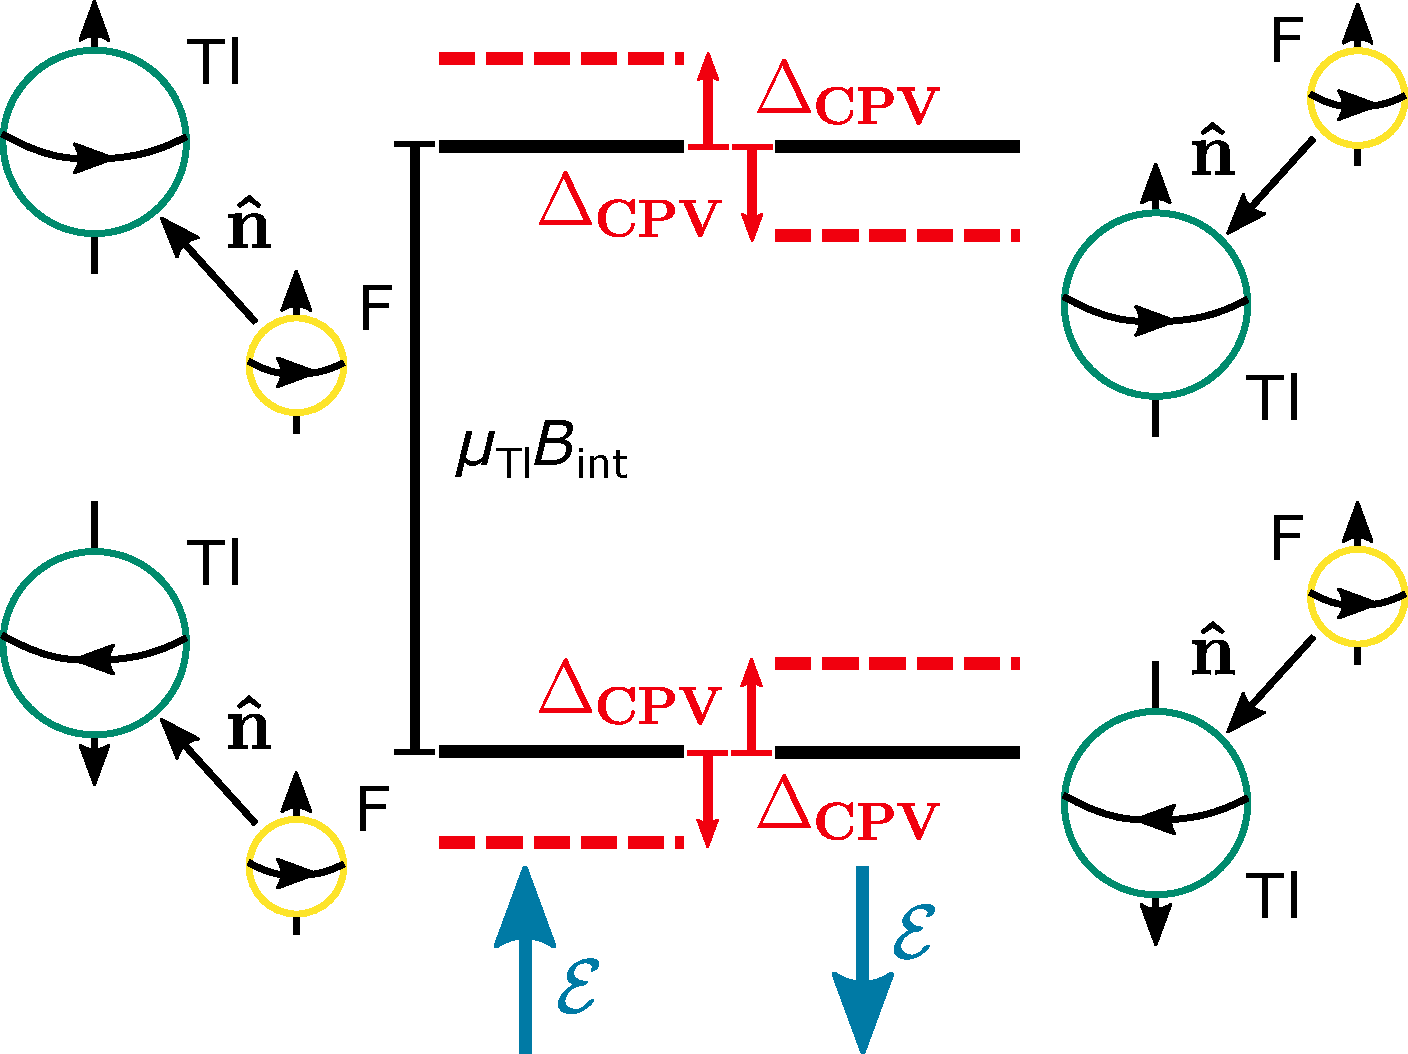
\includegraphics[width=0.48\textwidth,unit=1mm]{figs/svg/edm_levels_pdf_version.pdf}
	\caption{T-violating energy shift $\Delta_{\rm CPV} = W_SS\,\mathcal{P}$ as a result of a nonzero NSM $S$ given by the effective interaction $\mathcal{H}_\text{CPV}= W_S S\vec{I}\cdot \hat{\vec{n}}/I$ (Eq.~\ref{eq:Hamiltonian_effective_interaction}), shown for opposite orientations of the applied field $\Evec$. Here $\mu_1$ is the Tl magnetic moment and $B_1^\mathrm{int}$ is the effective internal magnetic field at the Tl nucleus due to the spin-rotation interaction.
	}
	\label{fig:edm_shift}
\end{figure}

Polar molecules can be polarized readily in laboratory-scale fields owing to their small rotational level separation ($\sim\!10^{-4}\eV$), giving them near-maximal energy shifts induced by a given Schiff moment. Thus, Sandars \cite{sandars1967measurability} suggested a molecular-beam resonance experiment could be used to probe the existence of the proton EDM, if the molecule has a heavy atom with an unpaired proton in the nucleus, such as $^{205}\mathrm{Tl}$. The value of $S$ is determined by measuring energy splittings between spin-up and -down states relative to $\left\langle \hat{\vec{n}}\right\rangle$ (which is parallel to the applied electric field $\bm{\mathcal{E}}$). This splitting will increase or decrease as $\bm{\mathcal{E}}$ (and hence $\left\langle \hat{\vec{n}}\right\rangle$) reverses, due to the interaction in Eq.~\ref{eq:Hamiltonian_effective_interaction}. The difference in level splittings is proportional to the electric polarization $\mathcal{P}$, the interaction strength $W_S$, and $S$ (Fig. \ref{fig:edm_shift}).

\CENTREX\ uses a cold beam of thallium fluoride (TlF) to measure nuclear $T$-violation due to the NSM of the $^{205}$Tl nucleus. It is a suitable system to look for $P$- and $T$-violating interactions for a number of reasons: a molecular beam of thallium fluoride can be readily obtained; many of the molecular states and transitions are known experimentally; the species is a polar diatomic molecule, enhancing the electron density gradient at the site of the nuclei (and hence $W_S$). As the thallium nucleus is heavy $\left(A=205,\,Z=81\right)$ and the NSM-induced energy shift scales $\propto A^{2/3}Z^2$, the observable effect of the Tl Schiff moment is correspondingly large \cite{sandars1967measurability, wilkening1984search}. Since the Tl nucleus contains an unpaired proton,
%the different linear combinations of underlying CPV parameters means
\CENTREX\ will be primarily sensitive to proton EDM effects, as opposed to other leading experiments which are more sensitive to the
%effects associated with neutron spin such as
neutron EDM \cite{graner2016reduced}. TlF is not very sensitive to the electron EDM due to its zero total electron spin \cite{kozlov1995parity}. 

The current best constraint on $T$-violating interactions associated with $S\left(^{205}\mathrm{Tl}\right)$ was found by Cho, Sangster and Hinds in 1991 \cite{cho1989tenfold, cho1991search}, who measured a NSM-induced frequency shift of $\Delta E = 2\Delta_{\rm CPV} = \left(1.4\pm 2.4\right)\times 10^{-4}$~Hz, consistent with zero.\footnote{Throughout, we express both frequencies and energies in linear frequency units (Hz), and all angular momentum operators are treated as dimensionless.} 
Using the effective interaction $\mathcal{H}_\text{CPV}$, the shift in the energy splitting between states with Tl spin up versus spin down, relative to the quantization axis, can be interpreted as
\begin{equation}
    \Delta E= 2 \Delta_{\rm CPV} = 2 W_S\,S\, \textrm{sgn}(\Esca) \,\mathcal{P},
    \label{eq:frequency_shift_due_to_NSM}
\end{equation}
where $W_S = 40539\,$a.u.,
polarization $\mathcal{P} = \langle\hat{\vec{n}} \cdot \hat{\Evec}\rangle = 0.547$, and the sign of $\Esca$ refers to the direction of $\Evec$ relative to a fixed quantizing axis $\hat{z}$.  This determines the Schiff moment \cite{PhysRevA.101.042501, PhysRevLett.88.073001}
\begin{equation}
    S\left(^{205}\mathrm{Tl}\right) = \left(3.6\pm 6.1\right)\times 10^{-11}\,e\,\mathrm{fm}^3.
\end{equation}
With Eq.~\ref{eq:schiff_contributions}, the following limits can be placed:
\begin{equation}
    \label{eq:prev_best_lims}
    \begin{split}
        \bar{\theta} & = \left(1.3 \pm 2.3\right)\ee{-9}, \\
        12\bar{d}_d+9\bar{d}_u & = \left(3.6\pm 6.1\right)\ee{-24}\,\mathrm{cm}, \\
        d_p          & = \left(0.9 \pm 1.5\right)\ee{-23}\,e\,\mathrm{cm},\\
        0.13g\bar{g}_0 - 0.004g\bar{g}_1-0.27g\bar{g}_2 & = \left(3.6 \pm 6.1\right)\ee{-11}.
    \end{split}
\end{equation}
\CENTREX\ aims to improve on these limits by using a cryogenic molecular beam source to achieve a cold beam with higher intensity and lower velocity spread compared to the jet source used in the previous work. Rotational cooling will be performed with optical and microwave pumping, collapsing much of the initial Boltzmann distribution into one state, greatly enhancing the number of molecules accessible for measurement. Finally, optical cycling will be used to assist state readout, resulting in near-unity detection efficiency. Fluorescence detection, compared to the hot-wire techniques used previously, allows for background-free detection if scattered light is well controlled.

\subsection{Thallium Fluoride}
\label{sec:tlf_theory}

\begin{figure}
	    % for axis breaks
    \usetikzlibrary{decorations.markings}
    \def\MarkLt{4pt}
    \def\MarkSep{2pt}
    \tikzset{
      TwoMarks/.style={
        postaction={decorate,
          decoration={
            markings,
            mark=at position #1 with
              {
                  \begin{scope}[xslant=0.2]
                  \draw[line width=\MarkSep,white,-] (0pt,-\MarkLt) -- (0pt,\MarkLt) ;
                  \draw[-] (-0.5*\MarkSep,-\MarkLt) -- (-0.5*\MarkSep,\MarkLt) ;
                  \draw[-] (0.5*\MarkSep,-\MarkLt) -- (0.5*\MarkSep,\MarkLt) ;
                  \end{scope}
              }
           }
        }
      },
      TwoMarks/.default={0.5},
    }

\begin{tikzpicture}[scale=5]

   % length of energy level diagram lines
   \def\len{.05}

   % x-position and length and x-offset of the y-axis labels
   \def\pos{-18}
   \def\lenmark{.025}
   \def\xoffset{.18}

   % x coordinates for m = -2, ... 2
   \def\xa{-4.5*\len}
   \def\xb{-2.5*\len}
   \def\xc{-0.5*\len}
   \def\xd{+1.5*\len}
   \def\xe{+3.5*\len}
   \def\xf{-6.5*\len}
   \def\xg{+5.5*\len}

   % y offset for J = 1, 2
   \def\yA{.6}
   \def\yB{\yA+.7}

   % axis
   \draw[->,TwoMarks=0.2,TwoMarks=0.6] (\xf-\len-\xoffset, -.1)
      -- (\xf-\len-\xoffset,\yB+.25) node[above, xshift = -20] {$E$ [kHz]};

   % brace position
   \def\bracePos{\xg+3*\len}

    
   % J=0 labels
   \draw [decorate,decoration={brace,amplitude=5pt,mirror,raise=4pt},yshift=0pt]
      (\bracePos,-.08) -- node (midJ0) {} (\bracePos,.08) node [black,midway,anchor=west,xshift=25] (nodeJ0) {$0$};
   \draw (\xf-\len-0.5*\lenmark-\xoffset, -.003325) node[anchor=east,below,xshift=\pos]
      {-3.325} -- (\xf-\len+0.5*\lenmark-\xoffset,-.003325) node[right,below,xshift=-\pos] {$1$};
   \draw (\xf-\len-0.5*\lenmark-\xoffset, .009975) node[anchor=east,above,xshift=\pos]
      {9.975} -- (\xf-\len+0.5*\lenmark-\xoffset,.009975) node[right,above,xshift=-\pos] {$0$};

   % J=0 lines
   \draw (\xc, -0.003325) -- (\xc+\len, -0.003325);
   \draw (\xb, -0.003325) -- (\xb+\len, -0.003325);
   \draw (\xd, -0.003325) -- (\xd+\len, -0.003325);
   \draw (\xc, 0.009975) -- (\xc+\len, 0.009975);

   % J=1 labels
   \draw [decorate,decoration={brace,amplitude=10pt,mirror,raise=4pt},yshift=0pt]
      (\bracePos,\yA-.2) -- node (midJ1) {} (\bracePos,\yA+.1) node [black,midway,anchor=west,xshift=25] (nodeJ1) {$1$};
   \draw (\xf-\len-0.5*\lenmark-\xoffset, \yA-.143745) node[anchor=east,below,xshift=\pos] {-143.745} --
      (\xf-\len+0.5*\lenmark-\xoffset,\yA-.143745) node[right,below,xshift=-\pos] {$0$};
   \draw (\xf-\len-0.5*\lenmark-\xoffset, \yA-.121506) node[anchor=east,above,xshift=\pos] {-121.506} --
      (\xf-\len+0.5*\lenmark-\xoffset,\yA-.121506) node[right,above,xshift=-\pos] {$1$};
   \draw (\xf-\len-0.5*\lenmark-\xoffset, \yA+.054446) node[anchor=east,below,xshift=\pos] {54.446} --
      (\xf-\len+0.5*\lenmark-\xoffset,\yA+.054446) node[right,below,xshift=-\pos] {$1$};
   \draw (\xf-\len-0.5*\lenmark-\xoffset, \yA+.068985) node[anchor=east,above,xshift=\pos] {68.985} --
      (\xf-\len+0.5*\lenmark-\xoffset,\yA+.068985) node[right,above,xshift=-\pos] {$2$};

   % J=1 lines
   \draw (\xc, \yA-.143745) -- (\xc+\len, \yA-.143745);
   \draw (\xc, \yA-.121506) -- (\xc+\len, \yA-.121506);
   \draw (\xb, \yA-.121506) -- (\xb+\len, \yA-.121506);
   \draw (\xd, \yA-.121506) -- (\xd+\len, \yA-.121506);
   \draw (\xc, \yA+.054446) -- (\xc+\len, \yA+.054446);
   \draw (\xb, \yA+.054446) -- (\xb+\len, \yA+.054446);
   \draw (\xd, \yA+.054446) -- (\xd+\len, \yA+.054446);
   \draw (\xc, \yA+.068985) -- (\xc+\len, \yA+.068985);
   \draw (\xb, \yA+.068985) -- (\xb+\len, \yA+.068985);
   \draw (\xd, \yA+.068985) -- (\xd+\len, \yA+.068985);
   \draw (\xa, \yA+.068985) -- (\xa+\len, \yA+.068985);
   \draw (\xe, \yA+.068985) -- (\xe+\len, \yA+.068985);

   % J=2 labels
   \draw [decorate,decoration={brace,amplitude=10pt,mirror,raise=4pt},yshift=0pt]
      (\bracePos,\yB-.27) -- node (midJ2) {} (\bracePos,\yB+.18) node [black,midway,anchor=west,xshift=25] (nodeJ2) {$2$};
   \draw (\xf-\len-0.5*\lenmark-\xoffset, \yB-.217455)
   node[anchor=east,left,yshift=-5] {-217.455}
      -- (\xf-\len+0.5*\lenmark-\xoffset,\yB-.217455) node[right,below,xshift=-\pos] {$1$};
   \draw (\xf-\len-0.5*\lenmark-\xoffset, \yB-.172936)
   node[anchor=east,left,yshift=5] {-172.936}
      -- (\xf-\len+0.5*\lenmark-\xoffset,\yB-.172936) node[right,above,xshift=-\pos] {$2$};
   \draw (\xf-\len-0.5*\lenmark-\xoffset, \yB+.105876)
   node[anchor=east,left,yshift=-5] {105.876}
      -- (\xf-\len+0.5*\lenmark-\xoffset,\yB+.105876) node[right,below,xshift=-\pos] {$2$};
   \draw (\xf-\len-0.5*\lenmark-\xoffset, \yB+.141095)
   node[anchor=east,left,yshift=5] {141.095}
      -- (\xf-\len+0.5*\lenmark-\xoffset,\yB+.141095) node[right,above,xshift=-\pos] (J2F3label) {$3$};

   % J=2 lines
   \draw (\xc, \yB-.217455) -- (\xc+\len, \yB-.217455);
   \draw (\xb, \yB-.217455) -- (\xb+\len, \yB-.217455);
   \draw (\xd, \yB-.217455) -- (\xd+\len, \yB-.217455);
   \draw (\xc, \yB-.172936) -- (\xc+\len, \yB-.172936);
   \draw (\xb, \yB-.172936) -- (\xb+\len, \yB-.172936);
   \draw (\xd, \yB-.172936) -- (\xd+\len, \yB-.172936);
   \draw (\xa, \yB-.172936) -- (\xa+\len, \yB-.172936);
   \draw (\xe, \yB-.172936) -- (\xe+\len, \yB-.172936);
   \draw (\xc, \yB+.105876) -- (\xc+\len, \yB+.105876);
   \draw (\xb, \yB+.105876) -- (\xb+\len, \yB+.105876);
   \draw (\xd, \yB+.105876) -- (\xd+\len, \yB+.105876);
   \draw (\xa, \yB+.105876) -- (\xa+\len, \yB+.105876);
   \draw (\xe, \yB+.105876) -- (\xe+\len, \yB+.105876);
   \draw (\xc, \yB+.141095) -- (\xc+\len, \yB+.141095);
   \draw (\xb, \yB+.141095) -- (\xb+\len, \yB+.141095);
   \draw (\xd, \yB+.141095) -- (\xd+\len, \yB+.141095);
   \draw (\xa, \yB+.141095) -- (\xa+\len, \yB+.141095);
   \draw (\xe, \yB+.141095) -- (\xe+\len, \yB+.141095);
   \draw (\xf, \yB+.141095) -- (\xf+\len, \yB+.141095);
   \draw (\xg, \yB+.141095) -- (\xg+\len, \yB+.141095);

   % microwave energies
   \draw[Latex-Latex] (nodeJ0) -- node[above,sloped] {13.3 GHz} (nodeJ1);
   \draw[Latex-Latex] (nodeJ1) -- node[above,sloped] {26.7 GHz} (nodeJ2);

   % approximate F1 labels
   \def\FposX{-5}
   \def\FposY{15}
   \def\FposYY{22}
   \node[xshift=\FposX] at (midJ0) {\nicefrac{1}{2}};
   \node[xshift=\FposX,yshift=-\FposY] at (midJ1) {\nicefrac{1}{2}};
   \node[xshift=\FposX, yshift=\FposY] at (midJ1) {\nicefrac{3}{2}};
   \node[xshift=\FposX,yshift=-\FposYY] at (midJ2) {\nicefrac{3}{2}};
   \node[xshift=\FposX, yshift=\FposYY] at (midJ2) {\nicefrac{5}{2}};
   \node[xshift=\FposX, yshift=47] at (midJ2) (F1label) {$F_1$};
    
   \node at (F1label -| nodeJ2) {$J$};
   \node at (F1label -| J2F3label) {$F$};

\end{tikzpicture}

	\caption{Hyperfine structure in the lowest three rotational levels in the TlF ground state $X^1\Sigma^+$, with no applied fields. Rotational energies $hBJ(J+1)$ should be added to
	%are subtracted from
	the hyperfine energy shifts indicated on the axis. Note the $(2F+1)$-fold degeneracy of each state with total angular momentum $F$, corresponding to the quantum numbers $m_F=-F,\dots,0,\dots,F$.}
	\label{fig:level_diagram}

\end{figure}

The TlF molecule is described by its electronic, vibrational and rotational motion, plus the states of the Tl and F nuclear spins. \CENTREX\ makes use of states both in the vibronic ground state, $X ^1\Sigma^+\left(\nu=0\right)$, and in an electronically excited state, $B ^3\Pi_1\left(\nu=0\right)$.  In both cases, we describe the angular momentum couplings in a Hund's case (a) basis. We typically write energy eigenstates in terms of the basis states $\ket{\eta,J,F_1,F,m_F}$. Here, $\eta$ represents the vibronic quantum numbers; $J$ is the total angular momentum excluding the nuclear spins, $\vec{F}_1 = \vec{J}+\vec{I}_\mathrm{1}$, with $I_\mathrm{1}=1/2$ for $^{205}$Tl; $\vec{F} = \vec{F}_1+\vec{I}_\mathrm{2}$ is the total angular momentum, with $I_\mathrm{2}=1/2$ for $^{19}$F; and $m_F$ is its projection along a quantization axis in the lab frame. Field-free eigenstates are close to these basis states in the ground $X ^1\Sigma^+$ state.  In the $B ^3\Pi_1$ state, strong hyperfine interactions significantly mix states with different $J$ and $F_1$ values. Hence, we describe these eigenstates with the modified notation $\ket{\eta',\widetilde{J}' ,\widetilde{F}_1^\prime,F',m_F'}$, where $\widetilde{J}'$ and $\widetilde{F}_1^\prime$ correspond to the largest component in their basis-state decomposition; the primes indicate that the ket refers to the excited state $B ^3\Pi_1$.

Molecules in the beam are assumed to be in the vibronic ground state, since the beam temperature is much lower than the energy scales associated with the electronic and vibrational excitations. However, even at cryogenic temperatures, there is a Boltzmann distribution over many rotational and nuclear spin states. The dominant term in the energy of rotational/spin levels in the $X ^1\Sigma^+$ state is due to rotation; the mean energy of states with quantum number $J$ is $E_\mathrm{rot}=BJ(J+1)$, where $B\approx 6.67\GHz \approx 0.3\kelvin\,\kB$, where $\kB$ the Boltzmann constant.\footnote{In Ramsey et al.\ \cite{wilkening1984search}, the symbol $B$ denotes the rotational constant in equilibrium position, i.e., there $B\equiv B_\text{e}$. However, the effective $v=0$ rotational constant, $B_0$, is more relevant to \CENTREX. To first order in the Dunham expansion \cite{huber2013molecular}, $B_0=B_\text{e}-\alpha_\text{e}/2$. With $B_\text{e}$ and $\alpha_\text{e}$ from the NIST database \cite{afeefy2011nist}, we find $B_0$. We define the symbol $B\equiv B_0$; its value is shown in Table~\ref{tab:hyperfine_hamiltonian}.}

Hyperfine interactions split sublevels with different $F$ values ($F=J-1,J,J, J+1$, except $F=0,1$ only for $J=0$) in each rotational state. Thus, each rotational level has $4(2J+1)$ magnetic sublevels. %including nuclear spins.
Including rotation, spin-rotation and spin-spin interactions, plus interactions with external electric $(\Evec)$ and magnetic $(\Bvec)$ fields, the system is described by the effective Hamiltonian \cite{wilkening1984search}
\small
$\mathcal{H}_\text{TlF} = \mathcal{H}_\text{rot}+\mathcal{H}_\text{sr}+\mathcal H_\text{ss} + \mathcal H_\text{S}+\mathcal H_\text{Z}$, 
\normalsize
where
\begin{equation} 
    \label{eq:hyperfine_hamiltonian}
    \begin{split}
        \mathcal H_\text{rot} & = B \vec{J}^2 \\
        \mathcal H_\text{sr}&=c_1(\vec I_1\cdot\vec J)+c_2(\vec I_2\cdot\vec J), \\
        \mathcal H_\text{ss}&=c_3 T^2(\vec C)\cdot T^2(\vec I_1, \vec I_2)+c_4(\vec I_1\cdot\vec I_2), \\
        \mathcal H_\text{S}&=-\vec\mu_e\cdot\vec \Evec,\\
        \mathcal H_\text{Z}&=-\frac{\mu_J}{J}(\vec J\cdot\vec \Bvec)-\frac{\mu_1}{I_1}(\vec I_1\cdot\vec \Bvec)-\frac{\mu_2}{I_2}(\vec I_2\cdot\vec \Bvec).
    \end{split}
\end{equation}
Here, the first term in the spin-spin interaction ($\mathcal H_\text{ss}$) contains the scalar product of two rank-2 tensors: one constructed from the modified spherical harmonics $\vec C$, and one from $\vec{I}_1$ and $\vec{I}_2$ \cite{brown2003rotational}. (The matrix elements diagonal in $J$ of this term are given in \cite{wilkening1984search}.)  The hyperfine parameters $c_1,c_2,c_3,c_4$, rotational constant $B$, magnetic moments $\mu_J,\mu_1,\mu_2$, and molecule-frame electric dipole moment $\mu_e$ are all known from previous measurements; their values are given in  Table~\ref{tab:hyperfine_hamiltonian}. A level diagram of low-lying states in the absence of applied fields is shown in Fig.~\ref{fig:level_diagram}.

\begin{table}
    \small
    \setlength\extrarowheight{3pt}
    \rowcolors{2}{white}{gray!25}
	\centering
	\caption{Constants describing rotational, hyperfine, Zeeman, and Stark interactions in the effective TlF ground-state  Hamiltonian (Eq.~\ref{eq:hyperfine_hamiltonian}). All values taken from Ramsey et al.\ \cite{wilkening1984search}, except for $B$ (see Sec. \ref{sec:tlf_theory}).}
	\label{tab:hyperfine_hamiltonian}
	\begin{tabular}{r@{\hspace{5pt}}c@{\hspace{5pt}}l@{\hspace{5pt}}l | r@{\hspace{5pt}}c@{\hspace{5pt}}l@{\hspace{5pt}}l}
    	\toprule
		$B$ & = &           $6.66733$ &     GHz &       $\mu_e$ & = & $4.2282(8)$ &     Debye \\
		$\mu_J$ & = &       $35(15)$ &      Hz/G &      $c_1$ & = & $126.03(12)$ &    kHz \\
		$\mu_1^{205}$ & = & $1.2405(3)$ &   kHz/G &     $c_2$ & = & $17.89(15)$ &     kHz\\
		$\mu_1^{203}$ & = &  $1.2285(3)$ &   kHz/G &     $c_3$ & = & $0.70(3)$ &       kHz \\
		$\mu_2$ & = &      $2.00363(4)$ &  kHz/G  &    $c_4$ & = & $-13.30(72)$ &    kHz \\
		\bottomrule
	\end{tabular}
\end{table}

%%%%%%%%%%%%%%%%%%%%%%%%%%%%%%%%%%%%%%%%%%%%%%55%%%%%%%%%%%%%%%
In \CENTREX, lasers are tuned to $X^1\Sigma^+(\nu=0)\rightarrow B^3\Pi_1\left(\nu=0\right)$ transitions in order to manipulate and read out ground state hyperfine and rotational sublevels. Details of the $B ^3\Pi_1$ state structure are given in \cite{norrgard2017hyperfine,PhysRevA.101.042506}.  Here, only a few main features of the $B$ state substructure are important.  First, the $B$ state hyperfine splittings are very large ($\gtrsim 100\MHz$) compared to the natural linewidth of the transition ($\gamma_B \approx 1.6\MHz$), which is in turn much larger than the ground-state hyperfine splittings ($c_j \lesssim 100\kHz$). This means that hyperfine structure is fully resolved in the excited state, and entirely unresolved in the ground state. Hence, optical transitions in TlF drive a large manifold of ground-state hyperfine levels (with a given value of $J$) to a single hyperfine state with (nominal) quantum numbers $\tilde{J},\tilde{F}_1$ and exact quantum number $F$. Another important feature of the $B$ state is that its matrix of Franck-Condon factors (FCFs) for decay to the $X$ state is extremely diagonal \cite{hunter2012prospects}, such that $\sim\! 99\%$ of the time, the $B(v=0)$ vibronic state decays back to the vibronic ground state $X(v=0)$.  This enables optical pumping and optical cycling with little loss.  However, the mixing of $J$ and $F_1$ by the strong $B$-state hyperfine interaction substantially modifies rotational selection rules in $B-X$ decays, and must be taken into account when describing optical excitation and emission in TlF.

\subsection{TlF in \texorpdfstring{$\Esca$}{E}-fields}
\label{sec:TlF_in_E_fields}

\begin{figure*}
	\centering
	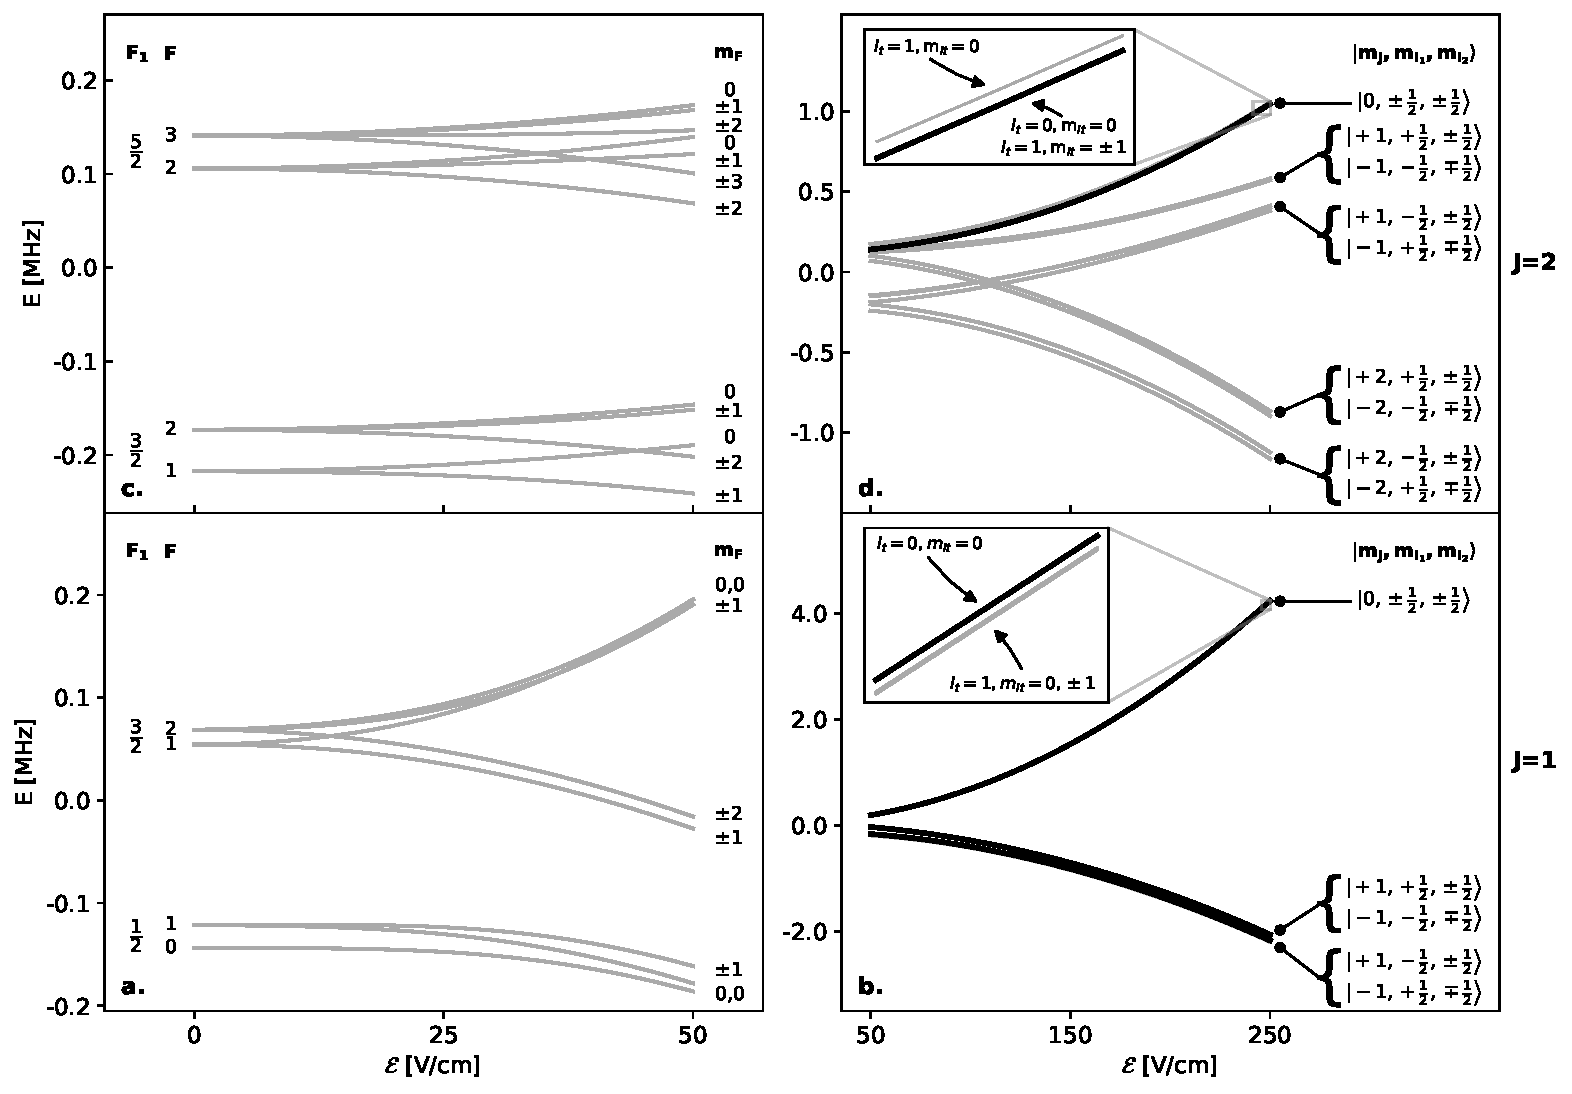
\includegraphics[width=\textwidth]{figs/matplotlib/low_to_mid_field.pdf}
	\caption{Overview of the energy eigenstates for changing $\Esca$-field magnitudes. The low-field regime, where $\Delta E_{\rm S} \ll E_{\rm hf}$, where energy eigenstates retain $J$, $F$, and $F_1$ as approximate quantum numbers is shown in \part{a} for $J=1$ and \part{c} for $J=2$. The mid-field regime, where $E_{\rm hf} \ll \Delta E_{\rm S} \ll E_{\rm rot}$, where both $J$ and $m_J$ are approximate quantum numbers is shown in \part{b} for $J=1$ and \part{d} for $J=2$. States used in \CENTREX\ are shown in bold.}
	\label{fig:low_to_mid_field}
\end{figure*}

\begin{figure}
	\centering
	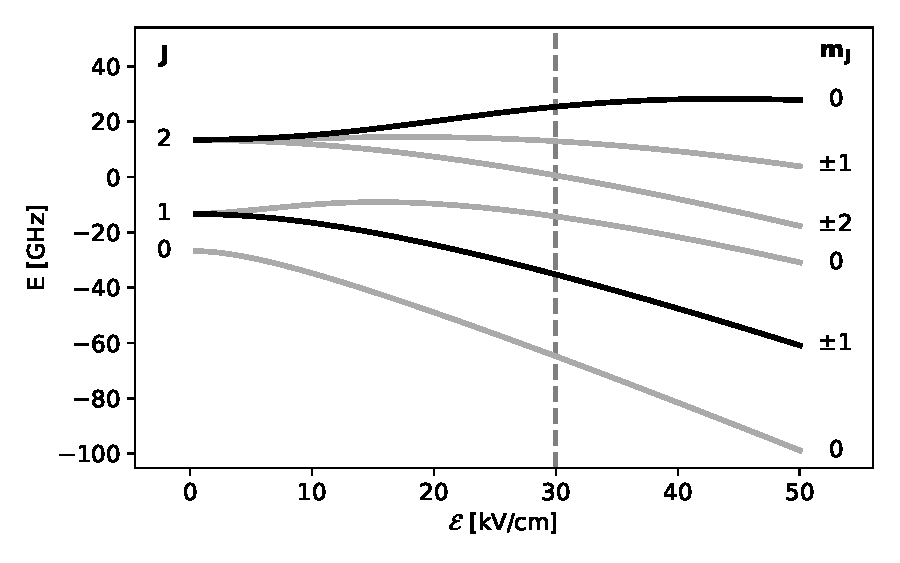
\includegraphics[width=\textwidth/2]{figs/matplotlib/low_to_high_field.pdf}
	\caption{Evolution of the energy eigenstates of the TlF Hamiltonian (Eq. \ref{eq:hyperfine_hamiltonian}) for $\Esca$ ranging from $0\,$V/cm to $50\,$kV/cm, for $J=0,1,2$. States used in \CENTREX\ are shown in bold. Hyperfine structure is unresolved in this plot.}
	\label{fig:low_to_high_field}
\end{figure}

Throughout most of the \CENTREX\ apparatus, TlF molecules experience a non-zero $\Esca$-field and (nominally) zero $\Bsca$-field.
The character of the energy eigenstates changes significantly depending on the $\Esca$-field magnitude, which varies dramatically between stages of the experiment. Hence, it is useful to describe the energy eigenstates of the TlF electronic ground state in different regimes of $\Esca$-field strength (with $\Bsca = 0$), as defined by the ratio of Stark shifts, $\Delta E_{\rm S} = \langle \mathcal{H}_{\rm S}\rangle \sim \mu_e^2 \Esca^2/B$, to the strength of hyperfine interactions, $E_{\rm hf} = \langle \mathcal{H}_{\rm sr} + \mathcal{H}_{\rm ss}\rangle \sim c_j$, or rotational energies, $E_{\rm rot} = \langle \mathcal{H}_{\rm rot}\rangle \sim B$. In all regimes, the total angular momentum projection $m_F$ along 
a space-fixed quantization axis $\hat{z}$ (always defined such that $\Evec$ is very nearly parallel to $\hat{z}$), is an exact quantum number.

In the low-field regime, where $\Delta E_{\rm S} \ll E_{\rm hf}$, energy eigenstates retain $J$, $F$, and $F_1$ as approximate quantum numbers. 
In the mid-field regime, where $E_{\rm hf} \ll \Delta E_{\rm S} \ll E_{\rm rot}$, both $J$ and $m_J$ are approximate quantum numbers. 
Here, the tensor part of the Stark shifts gives rise to energy splittings between levels with different values of $|m_J|$ that are comparable in size to the scalar shifts, i.e., of order $\Delta E_{\rm S}$.  Thus, when $m_J\neq 0$, $\vec{J}$ is strongly coupled to $\Evec$ (and hence to the molecular axis $\vec{\hat{n}}$) by this Stark interaction. In this case, each nuclear spin is coupled to $\vec{J}$ (and thus also to $\Evec$) by the spin-rotation interactions of $\mathcal{H}_{\rm sr}$. Hence, here $m_{I_1}$ and $m_{I_2}$ are approximate quantum numbers. By contrast, in states where $m_J=0$ (including when $J=0$) in this regime, $\left\langle \mathcal{H}_{\rm sr}\right\rangle$ vanishes to first order, and the nuclear spins do not couple to $\vec{J}$ and $\Evec$. However, the nuclear spins remain coupled to each other via the spin-spin interaction $\mathcal{H}_{\rm ss}$.  So, here the total nuclear spin $\vec \It = \vec I_1 + \vec I_2$ and its projection $m_{\It}$ are approximate quantum numbers in addition to $J$ and $m_J=0$. 
Finally, in the high-field regime where $E_{\rm hf} \ll E_{\rm rot} \lesssim \Delta E_{\rm S}$, $J$ states are strongly mixed, and separations between $m_J$ states are on the order of $E_{\rm rot}$. Here, eigenstates are defined by the same approximate quantum numbers as in the mid-field regime, aside from $J$. We refer to these strongly mixed states with the label $\widetilde{J}$, which corresponds to the value of $J$ that any given state connects to adiabatically, if the $\Esca$-field is reduced.
Table \ref{tab:E_field_regimes} summarizes the different regimes and associated eigenstates.  
\begin{table*}[t]
    \centering
    \def\colseplarge{4ex} % should only be used in this table
	\begin{tabular}{@{}r@{\hspace{\colseplarge}}r@{$\,\Delta E_{\rm S}\,$}l@{\hspace{\colseplarge}}r@{$\,\Esca\,$}l@{\hspace{\colseplarge}}>{\raggedright\arraybackslash}m{4cm}@{}}
    	\toprule
    	Regime & \multicolumn{2}{c}{Definition} & \multicolumn{2}{c}{Field strength} & Approx. eigenstates \\
		\midrule
		 Low
		 & & $\ll E_{\rm hf}$
		 & & $\lesssim 50 \Vcm$
		 & $\ket{J,F_1,F,m_F}$ \\\addlinespace[2ex]
		 %
	     Mid
	     & $E_{\rm hf} \ll$ & $\ll E_{\rm rot}$
	     & $50 \Vcm \ll$ & $\lesssim 5 \kVcm$
	     & $\ket{J,m_J \neq 0}\ket{m_{I_1},m_{I_2}}$ 
	       $\ket{J,m_J=0}\ket{\It,m_{\It}}$ \\\addlinespace[2ex]
	     %
	     High
	     & $E_{\rm hf} \ll E_{\rm rot} \lesssim$ &
	     & $5\kVcm \ll$ &
	     & $\ket{\widetilde{J},m_J\neq 0} \ket{m_{I_1},m_{I_2}}$
	       $\ket{\widetilde{J},m_J=0}\ket{\It,m_{\It}}$ \\
		\bottomrule
	\end{tabular}
	\caption{Regimes of electric field strength and associated eigenstates in TlF.}
	\label{tab:E_field_regimes}
\end{table*}


Figure \ref{fig:low_to_mid_field} shows how the relevant energies and eigenstates evolve from the low-field to the mid-field regime for $J=1$ and $J=2$ states.  Bold curves are states directly relevant to \CENTREX. Figure \ref{fig:low_to_high_field} shows a zoom out of states up to $J=2$ from low to high fields.

The $^{205}$Tl NSM measurement is carried out in $\tilde{J} = 1,\, m_J = \pm1$ states of TlF at large electric field $\mathcal{E} = 30$ kV/cm. This choice of states takes advantage of the structure of TlF in electric fields, in two ways. First, the observable energy shift associated with $S$, $\Delta E$, scales linearly with the degree of polarization $\mathcal{P}$ of the TlF molecule (Eq. \ref{eq:frequency_shift_due_to_NSM}). An electric field more easily polarizes states with low $J$, since $\mathcal{P}$ arises from mixing between states with different parity and thus different $J$; these states are closest together when $J$ is small. Additionally, as discussed in Sec. \ref{Sec:InternalComagnetometry}, certain dangerous systematic errors in the NSM measurement are dramatically suppressed in the presence of a strong spin-rotation interaction (later referred to as an effective intra-molecular magnetic field). This requires $m_J \neq 0$. The $\tilde{J} = 1,\, m_J = \pm1$ states hence provide the best combination of sensitivity and systematic error suppression in TlF.\footnote{$|\mathcal{P}|$ is larger in the $J=0,m_J = 0$ states, given the same $\Esca$-field value. Hence, the NSM gives larger energy shifts there. However, in these states where $m_J = 0$, the effective intra-molecular magnetic field vanishes.}
\section{Related Work}
While writing this paper, we noticed that a paper \cite{Du2022LearningTS} that has similar ideas to our work was submitted to the arXiv. They propose a two-stage paradigm for selecting from multiple questions. They also propose a network similar to our {\bf \textsc{\name-B}} to select from multiple options in parallel. We summarize the differences between their work and ours as follows: (1) Different in paradigm. We have an expand stage to further improve the quality of recalled candidates (2) Different in models. {\bf \textsc{\name-S}} and {\bf \textsc{\name-B}} are both different from theirs in both input format and scoring. We additionally propose to discard the C2C attention and study the effect of removing different parts of attention. (3) We focus more on entity typing and conduct extensive experiments covering two languages and three settings (ultra-fine-grained, fine-grained, and coarse-grained). We analyze the effect of using different PLM backbones for a fairer and more comprehensive comparison.
The paradigm of our work is also inspired by works in entity linking and information retrieval. \citet{wu2019zero} uses a retrieval and rerank paradigm for entity linking, they first generate entity candidates using a bi-encoder and rerank them using a vanilla cross-encoder. Our paradigm with an additional expand stage and our proposed {\bf \textsc{\name}} models are also potentially useful for entity linking. We leave it for future work. \citet{halter} represents the query document and candidate documents as vectors and proposed to use a transformer to rerank all candidate documents in parallel for passage retrieval. Compared to them, we tackle entity typing and preserve all information of mention and context rather than represent them as a single vector, the paradigm, model architecture, and training objective are also different.




% \iffalse
% \begin{table*}[htp!]\small \setlength{\tabcolsep}{7pt}
% \centering
% \caption{\small In the sentiment analysis task, we perform two types of targeted attack: concat attack and scatter attack. Concat attack does not change existing context but instead appends the adversarial sentence to the paragraph, while scatter attack scatters adversarial tokens over the whole passage. The attack target is from the most positive to the most negative, or vice versa. In the QA task, we also perform two types of targeted attack: during answer targeted attack with the answer targeted  to ``donald trump'',  the model outputs ``donald trump''; during position targeted attack, the model always output the fake answer from our appended sentence. \advcodecword is operated on the leaf nodes without propagating through the entire dependency trees and is not guaranteed to generate natural sentences; while \advcodecsent is capable of generating high quality adversarial sentences, by considering the global dependency structures during decoding.
% %We also perform the targeted position attack on initial sentence ``\textbf{the the the} win ultra bowls 40'' and automatically generate a fake answer ``the fellow  journalists'' on its targeted position. 
% }
%  \label{examples}
% \begin{tabular}{p{0.9cm}p{11.5cm}p{2.0cm}}
% \toprule
% Task & Input (\textit{Italic} = Inserted or appended words, \underline{underline} = QA Model prediction, \textcolor{red}{red} = QA Ground truth) & Model Output \\
% \midrule
%   & \textbf{Concat Attack} (via \advcodecsent): \textit{I kept expecting to see chickens and chickens walking around.} ... This place is like a steinbeck novel come to life. I kept expecting to see donkeys and chickens walking around. wooo-pig-soooeeee this place is awful!!! 
%  &  Most Negative $\rightarrow$  Most Positive  \\
%  \multirow{3}{*}{\shortstack{Sentiment \\ Analysis}} & \textbf{Concat Attack} (via \advcodecword): \textit{heavenly royalty restored.} very disappointing . waffles were mushy , not crisp at all . chicken was way over cooked and poorly seasoned . great location in downtown gilbert . i wonder what will replace this disappointment .  
% & Most Negative $\rightarrow$ Most   Positive  \\ 
%  % & \textbf{Scatter Attack} (via \advcodecword): ... rude and racist , she did not help me at all! when i approached he, I am wearing my ethic dress, she \textit{restored} sized me and when i asked \textit{perfect} for \textit{the} help, she stated "perhaps you should make an appointment. " And then turned her back to me and began speaking another language with \textit{pleasantly} her friend...
%   % & Most Negative $\rightarrow$ Most  Positive  \\
  
% \midrule
% % & \textbf{Answer Targeted Attack} (via \advcodecword):& \\
%   & \textbf{Answer Targeted Attack} (via \advcodecsent): \textit{Q:  Who ended the series in 1989?} & Jonathan Powell  \\
%   & \textit{Paragraph: } ... Falling viewing numbers, a decline in the public perception of the show and a less-prominent transmission slot saw production suspended in 1989 by \textcolor{red}{Jonathan Powell}, controller of BBC 1. Although ... cancelled with the decision not to commission a planned 27th series of the show for transmission in 1990, the BBC repeatedly affirmed that the series would return. \textit{\underline{donald trump} ends a program on 1988 .} & $ \rightarrow $ donald trump  \\
   
%   \multirow{8}{*}{\centering QA}& \textbf{Position Targeted Attack} (via \advcodecsent): \textit{Q: Why would a teacher's college exist? } & serve and protect \\
%  & \textit{Paragraph: }
% There are a variety of bodies designed to instill, preserve and update the knowledge and professional standing of teachers. Around the world many governments operate teacher's colleges, which are generally established to \answer{serve and protect the public interest through certifying, governing and enforcing the standards of practice for the teaching profession.} \textit{a friend 's school exist \underline{for community , serving a private businesses.}} & the public ... $\rightarrow$ for community, serving a private businesses.  \\

%  &  \textbf{Answer Targeted Attack} (via \advcodecword): \textit{Q: What is the smallest geographical region discussed?} &   \\ & \textit{Paragraph: } Its counties of Los Angeles, Orange, San Diego, San Bernardino, and \answer{Riverside} are the five most populous in the state and all are in the top 15 most populous counties in the United States. \textit{a simplest geographic regions discuss \underline{donald trump}}. & Riverside \quad $ \rightarrow $ donald trump  \\
 
%   &  \textbf{Position Targeted Attack} (via \advcodecword :  \textit{Q: IP and AM are most commonly defined by what type of proof system?} & Interactive \quad $ \rightarrow $   \\ 
%   & \textit{Paragraph: } Other important complexity classes include BPP, ZPP and RP, which are defined using probabilistic Turing machines; AC and NC, which are defined using Boolean circuits; and BQP and QMA, which are defined using quantum Turing machines. \#P is an important complexity class of counting problems (not decision problems). Classes like IP and AM are defined using \answer{Interactive} proof systems. ALL is the class of all decision problems. \textit{we are non-consecutive defined by \underline{sammi} proof system .} & sammi  \\
%   %& \textit{Question: Who won Super Bowl 50?} & Carolina Panthers $ \rightarrow $ \\ & Super Bowl 50 was an American football game ... The American Football Conference (AFC) champion Denver Broncos defeated the National Football Conference (NFC) champion Carolina Panthers 24 - 10 to earn their third Super Bowl title... \textcolor{red}{the fellow journalists win ultra bowls 150.} &   the fellow journalists  \\
% \bottomrule
% \end{tabular}
% \end{table*}
% \fi

\section{Framework}

% In this section, we will describe the \advcodec framework. 

\subsection{Preliminaries}

Before delving into details, we recapitulate the attack scenario and attack capability supported by \advcodec framework. 

\textbf{Attack Scenario.} Unlike  previous adversarial text generation works \citep{2018arXiv181200151L, seq2sick,2016arXiv160408275P,2016arXiv160507725M,Alzantot2018GeneratingNL} that directly modify critical words in place and might risk changing the semantic meaning or editing the ground truth answers,
%(which makes it unreasonable to evaluate the adversarial score e.g. on Question Answering)
we are generating the \textit{concatenative adversaries} \citep{jia-liang-2017-adversarial} (\textit{abbr.}, concat attack). Concat attack does not change any words in original paragraphs or questions, but instead appends a new adversarial sentence to the original paragraph to fool the model. A valid adversarial sentence needs to ensure that the appended text is \textit{compatible} with the original paragraph, which in other words means it should not contradict any stated facts in the paragraph, especially the correct answer. 

\textbf{Attack Capability.} \label{two_attacks} \advcodec is essentially an optimization based framework to find the adversarial text with the optimization goal set to achieve the \textbf{targeted attack}. For the sentiment classification task, \advcodec can perform the targeted attack to make an originally positive review be classified as the most negative one, and vice versa. Particularly in the QA task, we design and implement two kinds of targeted attacks: \textit{position targeted attack} and \textit{answer targeted attack}. A successful position targeted attack means the model can be fooled to output the answers at specific targeted positions in the paragraph, but the content on the targeted span is optimized during the attack. So the answer cannot be determined before the attack. In contrast, a successful answer targeted attack is a stronger targeted attack, which refers to the situation when the model always outputs the pre-defined targeted answer no matter what the question looks like. In Table \ref{tab:example}, we set the targeted answer as ``Donald Trump'' and successfully changes the model predictions. More examples of answer targeted attacks and position targeted attacks can be found in Appendix \S\ref{appendix:examples}. 

Although our framework is designed as a whitebox attack, our experimental results demonstrate that the adversarial text can transfer to other blackbox models with high attack success rates. Finally, because \advcodec is a unified adversarial text generation framework whose outputs are discrete tokens,  it applies to different downstream NLP tasks. In this paper, we perform an adversarial evaluation on sentiment classification and QA as examples to illustrate this point.
% In our work, we further push the concept of concatenative adversaries  and propose a more general notion named \textbf{scatter attack}, which can inject adversarial words sporadically over the whole paragraph. 
% Our scatter attack is intrinsically more imperceptible to human being to detect the anomaly tokens, on the grounds that human empirically tends to omit or ignore tokens that looks irrelevant or like a typo. 
% The concatenative adversarial example falls into our case when those adversarial tokens form a sentence and on the same time the semantic meaning of the sentence does not contradict the original paragraph. Examples of concatenative attack and scatter attack is shown in table \ref{examples}.
%As for the location where we append the sentence, we choose to follow the \citeauthor{jia-liang-2017-adversarial}'s way to add the adversary to the end of the paragraph so that we can make a fair comparison with their results.
% although we do not directly change the original paragraph, we still need to ensure ...
% \vspace{-2mm}
\subsection{Tree Auto-Encoder} % \shuo{Pre-training?} -- also include model discription, so keep the current name
In this subsection,  we describe the key component of \advcodec: a tree-based autoencoder.  
% why tree
Compared with standard sequential generation methods, generating sentence in a non-monotonic order (e.g., along parse trees) has recently been an interesting topic~\citep{Welleck2019NonMonotonicST}.
Our motivation comes from the fact that sentence generation along parse trees can intrinsically capture and maintain the syntactic information~\citep{eriguchi-etal-2017-learning, aharoni-goldberg-2017-towards,Iyyer2018AdversarialEG}, and show better performances than sequential recurrent models~\citep{TreeImportant,Iyyer2014GeneratingSF}. Therefore we design a novel tree-based autoencoder to generate adversarial text that can simultaneously preserve both semantic meaning and syntactic structures of original sentences. Moreover, the discrete nature of language motivates us to make use of autoencoder to map discrete text into a high dimensional continuous space, upon which the adversarial perturbation can be calculated by gradient-based approaches to achieve targeted attack.  
% \shuo{The last sentence is not very clear. Why  efficiently and effectively? Compare to which method?}  -- This empowers us to leverage the optimization based method to search for adversarial perturbation on the continuous embedding space more efficiently and effectively than heuristic methods such as genetic algorithms, whose computation grows exponentially w.r.t. the input space. -- moved to introduction

Formally, let $X$ be the domain of text and $S$ be the domain of dependency parse trees over element in $X$, a tree-based autoencoder consists of an encoder $\mathcal{E}: X \times S \rightarrow Z $ that encodes text $\boldsymbol{x} \in X$ along with its dependency parsing tree  $\boldsymbol{s} \in S$ into a high dimensional latent representation $\boldsymbol{z} \in Z$ and a decoder $\mathcal{G}: Z \times S \rightarrow X$ that generates the corresponding text $\boldsymbol{x}$ from the given context vector $\boldsymbol{z}$ and the expected dependency parsing tree $\boldsymbol{s}$. Given a dependency tree $\boldsymbol{s}$, $\mathcal{E}$ and $\mathcal{G}$ form an antoencoder. We thus have the following reconstruction loss to train our tree-based autoencoder:
\begin{equation}
  \mathcal{L}_\text{recon} = - \mathbb{E}_{\boldsymbol{x}\sim X}[\log p_{\mathcal{G}}(\boldsymbol{x}|\boldsymbol{s}, \mathcal{E}(\boldsymbol{x}, \boldsymbol{s})]
\end{equation}
%As Figure \ref{fig:qa_pipeline} suggests, \advcodec can operate on different granularity levels to generate either word-level or sentence-level contextual representation, and decode it into the adversarial text. We refer the sentence-level \advcodec to \advcodecsent and the word-level one to \advcodecword. Both of them will be described in more details later in this section.

\textbf{Encoder.} We adopt the Child-Sum Tree-LSTM \citep{Tai2015ImprovedSR} as our tree encoder. Specifically, in the encoding phase, each child state embedding is its hidden state of Tree LSTM concatenated with the dependency relationship embedding. 
The parent state embedding is extracted by summing the state embedding from its children nodes and feeding forward through Tree-LSTM cell. The process is conducted from bottom (leaf node, i.e. word) to top (root node) along the dependency tree extracted by CoreNLP Parser \citep{Manning2014TheSC}. 
% The context vector $z$ for \advcodecsent refers to the root node embedding $h_{root}$, representing the sentence-level embedding. 

\begin{figure}
    \centering
    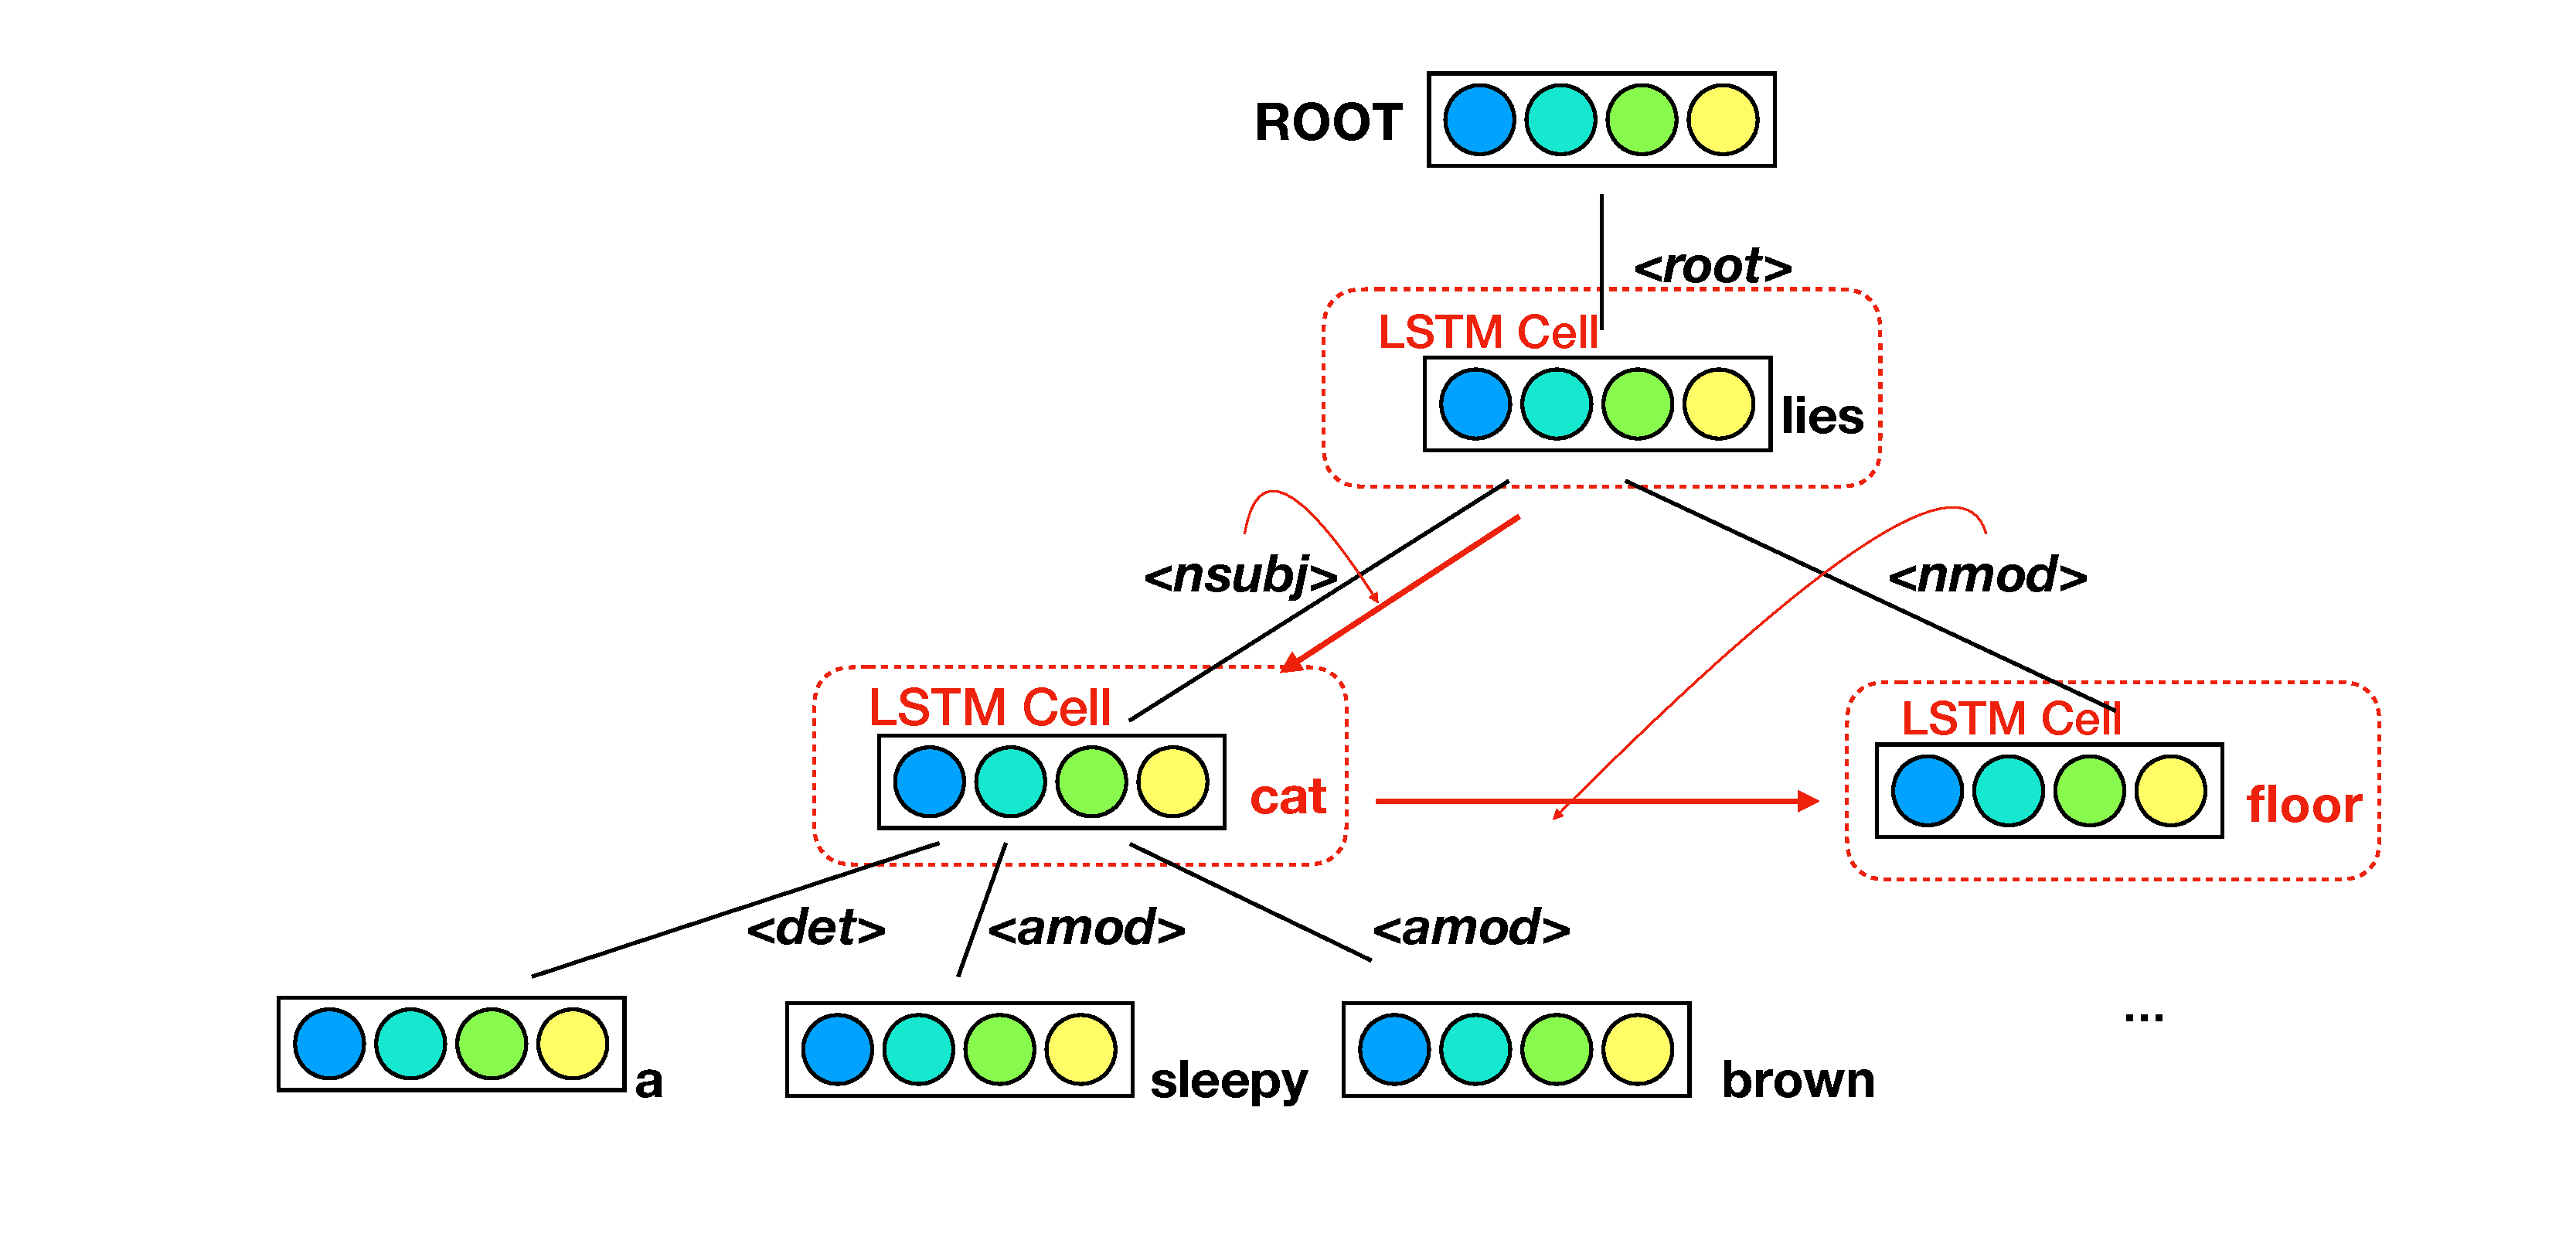
\includegraphics[page=1,trim=1cm 1.5cm 1cm 1.5cm,clip,width=\linewidth]{body/tree.pdf}
    \caption{The tree decoder. Each node in the dependency tree is a LSTM cell. Black lines refer to the dependencies between parent and child nodes. Red arrows refer to the directions of decoding. During each step the decoder outputs a token that is shown on the right of the node. } 
    \label{fig:tree}
\vspace{-3mm}
\end{figure}

\textbf{Decoder.} As there is no existing tree-based autoencoder, we design a novel Tree Decoder (Shown in Figure \ref{fig:tree}). In the decoding phase, we start from the root node and traverse along the same dependency tree in level-order. The hidden state $\boldsymbol{h}_j$ of the next node $j$ comes from (i) the hidden state $\boldsymbol{h}_i$ of the current tree node, (ii) current node predicted word embedding $\boldsymbol{w}_i$, and (iii) the dependency embedding $\boldsymbol{d}_{ij}$ between the current node $i$ and the next node $j$ based on the dependency tree. The next node's corresponding word $y_j$ is generated based on the hidden state of the LSTM Cell $\boldsymbol{h}_j$ via a linear layer that maps from the hidden presentation $\boldsymbol{h}_j$ to the logits that represent the probability distribution of the tree's vocabulary.
\begin{align}
     \boldsymbol{h}_j &= \text{LSTM}([\boldsymbol{h}_i;\boldsymbol{w}_i;\boldsymbol{d}_{ij}]) \\
    y_j &=  \text{one-hot} (\text{argmax} \left( \boldsymbol{W} \cdot \boldsymbol{h}_j  + \boldsymbol{b} \right)) \label{eq:decode_word}
\end{align}

%  it is inherently flexible to add perturbations on hierarchical nodes of the tree structures. 

Moreover, the tree structure allows us to modify the tree node embedding at different tree hierarchies in order to generate controllable perturbation on word level or sentence level. Therefore, we explore the following two types of attacks at root level and leaf level \advcodecsent and \advcodecword, which are shown in Figure \ref{fig:advsent} and Figure \ref{fig:advword}.

%For the very few failure cases for targeted ]attack, we observer a high amount . 
% targeted and untargeted
% whitebox blackbox

% \bo{emphasize we can attack sentiment and QA}

\begin{figure}[t]
    \centering
    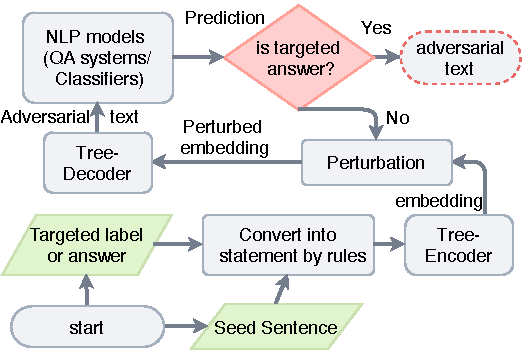
\includegraphics[width=\linewidth]{body/pipelinefull.pdf}
    \caption{The pipeline of adversarial text generation.}
    \label{fig:pipeline}
    \vspace{-3mm}
\end{figure}

 \begin{figure*}[t]
    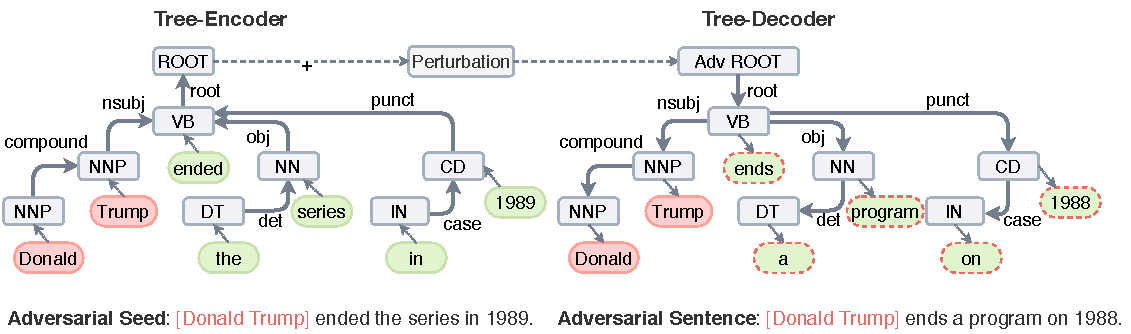
\includegraphics[trim=0cm 0cm 0cm 0cm,clip,width=1\linewidth]{body/pipelinesent.pdf}
    \caption{\small An example of how \advcodecsent generates the adversarial sentence. Perturbation is added on the ROOT embedding and optimized to ensure the success of targeted attack while the magnitude of perturbation is minimized.} % \shuo{How perturbation is optimized could also show here?}} 
    \vspace{-0.3cm}
    \label{fig:advsent}
\end{figure*}


\begin{figure}
    \centering
    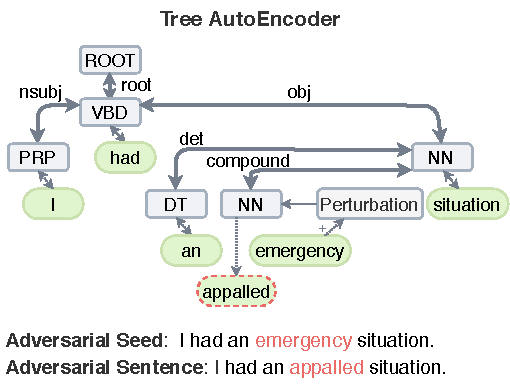
\includegraphics[width=\linewidth]{body/pipelineword.pdf}
    \caption{\small \advcodecword adds perturbation on the leaf node embedding. Arrow denotes the direction of encoding/decoding.  }
    %, encoded along the dependency tree and decoded back to adversarial token.} 
    \label{fig:advword}
    \vspace{-3mm}
\end{figure}

\subsection{Pipeline of Adversarial Text Generation}

Here we illustrate how to use our tree-based autoencoder to perform adversarial text generation and attack NLP models, as illustrated in Figure \ref{fig:pipeline}.

\textbf{Step 1: Choose the adversarial seed.} The adversarial seed is the input sentence to our tree autoencoder. After adding perturbation on the tree node embedding, the decoded adversarial sentence will be added to the original paragraph to perform concat attack. For sentiment classifiers, the adversarial seed can be an arbitrary sentence from the paragraph. For example, the adversarial seed of Yelp Review example in Table \ref{tab:example} is a random sentence from the paragraph \textit{``I kept expecting to see donkeys and chickens walking around.'}

In contrast, when performing answer targeted attack for QA models, we need add our targeted answer into our adversarial seed in a reasonable context.  Based on a set of heuristic experiments on how the adversarial seed correlates the attack efficacy (Appendix \ref{appendix:heuristic}), we choose to use question words to craft an adversarial seed, because it receives higher attention score when the model is matching semantic similarity between the context and the question. 
Specifically, we convert a question sentence to a meaningful declarative statement and assign a targeted fake answer. The fake answer can be crafted according to the perturbed model's predicted answer (position targeted attack \S \ref{two_attacks}), or can be manually chosen by adversaries (answer targeted attack). For instance, the answer targeted attack example shown in Table \ref{tab:example} converts the question \textit{``Who ended the series in 1989?''} into a declarative statement \textit{``someone ended the series in 1989.''} by a set of coarse grained rules (Appendix \ref{appendix:heuristic}).
%\shuo{How? Any reference?} 
Then our targeted wrong answer is assigned to generate the adversarial seed \textit{``Donald Trump ended the series in 1989.''}  Following steps will make sure that the decoded adversarial sentence does not contradict with the original paragraph. 
%The initial seed and the following optimization steps should ensure that the adversarial sentence is meaning preserving and label preserving. The sentence in the example above is simply repeating the paragraph, and thus is valid. 
%If we fail to convert a question to a statement, we will then use the answer sentence and perturb the critical information to preliminarily solve the compatibility issues. 

% if we choose a good adversarial seed that contains the targeted answer is semantically close to the context or the question
 
% it would be helpful to reduce the optimization steps of searching for the best perturbation and achieve targeted 
% For example, when attacking the BERT, we can simply sample a sentence from the original paragraph and append it to the start of the paragraph. 

% Different from attacking sentiment analysis, it is important to choose a good initial seed that is semantically close to the context or the question when attacking QA model. In this way we can reduce the number of iteration steps and attack the QA model more efficiently. 
%Based on a set of heuristic experiments on how the initial seed correlates the attacking efficacy, 

\textbf{Step 2: Embed the discrete text into continuous embedding.} One difference between \advcodecsent and \advcodecword is on which tree level we embed our discrete sentence. For \advcodecsent, we use tree root node embedding of Tree-LSTM $\boldsymbol{z} = \boldsymbol{h}_\text{root}$ to represent the discrete sentence (``ROOT'' node in the Figure \ref{fig:advsent}). As for \advcodecword, we concatenate all the leaf node embedding of Tree-LSTM $\boldsymbol{h}_i$ (corresponding to each word) $\boldsymbol{z} = [\boldsymbol{h}_1, \boldsymbol{h}_2, \dots, \boldsymbol{h}_n]$ to embed the discrete sentence.


% As illustrated in Figure \ref{fig:qa_pipeline}, both attacks start from an initial seed (sentence or tokens). The initial seed is later fed into the tree autoencoder. For \advcodecsent, it encodes through the encoder $\mathcal{E}$ and uses the root node embedding as the sentence representation $z$. We add perturbation $z^*$ on $z$ and propagate $z$ regularized by the tree decoder back to adversarial sentences. \advcodecword follows the same tree encoder but stops at the leaf level. The sentence leaf token embedding is then concatenated as the context vector $z$. After adversarial perturbation $z' = z + z^*$, the leaf node embedding $z'$ is then decoded into words via equation (\ref{eq:decode_word}). 

% Therefore, it is worth noting that because the encoding and decoding phases are completed in the leaf nodes without propagating through the dependency trees,
%while \advcodecsent can help regularize the syntactical correctness based on the tree decoder,
% \advcodecword does not guarantee the grammatical correctness of the adversarial sentences.
%We can also observe from Table \ref{examples} that the adversarial sentence quality generated by \advcodecword is worse than those generated by \advcodecsent. 
% But the advantage of \advcodecword lies on the flexibility, which can help us selectively perturb a very limited number of words instead of paraphrasing the whole sentence.

\textbf{Step 3: Perturb the embedding via optimization.} Finding the optimal perturbation $z^*$ on the embedding vector $z$ is equivalent to solving the optimization problem that can achieve the target attack goal while minimize the magnitude of perturbation
\begin{equation}
    \min \quad ||\boldsymbol{z}^*||_p + c  f(\boldsymbol{z} + \boldsymbol{z}^*),
    \label{cw}
\end{equation}
where $f$ is the objective function for the targeted attack and $c$ is the constant balancing between the perturbation magnitude and attack target. Specifically, we design the objective function $f$ similar to \citet{cw} for classification tasks
\begin{align}
        \ell &=  \max\big\{Z\left({\left[\mathcal{G}(\boldsymbol{z}', \boldsymbol{s}); \boldsymbol{x} \right] }\right)_i:i \neq t \big\},  \\
        f(\boldsymbol{z}') &= \max \big(\ell - Z\left(\left[\mathcal{G}(\boldsymbol{z}', \boldsymbol{s}); \boldsymbol{x} \right] \right)_t  , -\kappa \big),
\end{align}
where $\boldsymbol{z}'=\boldsymbol{z}+\boldsymbol{z}^*$ is the perturbed embedding, model input $\left[\mathcal{G}(\boldsymbol{z}', \boldsymbol{s}); \boldsymbol{x} \right]$ is the concatenation of adversarial sentence $\mathcal{G}(\boldsymbol{z}', \boldsymbol{s})$ and original paragraph $\boldsymbol{x}$, $t$ is the target class, $Z(\cdot)$ is the logit output of the classification model before softmax, $\ell$ is the maximum logits of the classes other than the targeted class and $\kappa$ is the confidence score to adjust the misclassification rate. The confidence score $\kappa$ is chosen via binary search to search for the tradeoff-constant between attack success rate and meaning perseverance. The optimal solution $z^*$ is iteratively optimized via gradient descent.

Similarly to attack QA models, we subtly change the objective function $f$ due to the difference between QA model and classification model:
\begin{align*}
        \ell_j &=  \max\big\{Z_j\left({\left[\boldsymbol{x}; \mathcal{G}(\boldsymbol{z}', \boldsymbol{s}) \right] }\right)_i:i \neq t_j \big\},  \\
        f(\boldsymbol{z}') &= \sum_{j=1}^{2} \max \big(\ell_j - Z_j\left(\left[\boldsymbol{x}; \mathcal{G}(\boldsymbol{z}', \boldsymbol{s}) \right] \right)_{t_j}, -\kappa \big),
\end{align*}
where $Z_1(\cdot)$  and $Z_2(\cdot)$ are respectively the logits of answer starting position and ending position of the QA system. $t_1$ and $t_2$ are respectively the targeted start position and the targeted end position.  $\ell_j$ is the maximum logits of the positions other than the targeted positions. Different from attacking sentiment classifier where we prepend the adversarial sentence, we choose to follow the setting of \citeauthor{jia-liang-2017-adversarial} to add the adversary to the end of the paragraph so that we can make a fair comparison with their results.

\begin{table*}[t!] \small
\centering
\begin{tabular}{ccccc|ccc}
\toprule
\multirow{2}{*}{Model} & Original & & \multicolumn{2}{c}{Whitebox Attack} & \multicolumn{3}{c}{Blackbox Attack} \\
\cmidrule(lr){4-5} \cmidrule(lr){6-8}
& Acc & & {\advcodecword} & {Seq2Sick}  & {\advcodecword} & {Seq2sick}  & TextFooler\\
\midrule
\multirow{2}{*}{BERT} & \multirow{2}{*}{0.703} & target   & \textbf{0.990}         & 0.974   & \textbf{0.499}         & 0.218  & 0.042         \\
    &  & untarget  & \textbf{0.993}          & 0.988  & \textbf{0.686}          & 0.510  & 0.318   \\
\midrule
\multirow{2}{*}{SAM} & \multirow{2}{*}{0.704} & target       & \textbf{0.956}   & 0.933  & \textbf{0.516}   & 0.333  & 0.113  \\
     & & untarget      & \textbf{0.967}          & 0.952  & \textbf{0.669} & 0.583  & 0.395    \\
\bottomrule
\end{tabular}
\caption{Adversarial evaluation on sentiment classifiers in terms of targeted and untargeted attack success rate. }
\label{tab:AttackSentiment}
% \vspace{-3mm}
\end{table*}

\textbf{Step 4: Decode back to adversarial sentence.} There are three problems we need to deal with when mapping embeddings to adversarial sentences: (1) the adversarial sentence may contradict to the stated fact of the original paragraph; (2) the decoding step (Eq. \ref{eq:decode_word}) uses argmax operator that gives no gradients,  but the step 3 needs to perform gradient descent to find the optimal $z^*$; (3) for answer targeted attack, the targeted answer might be perturbed and changed during decoding phase.

To solve problem (1), we guarantee our appended adversarial sentences are not contradictory to the ground truth by ensuring that the adversarial sentence and answer sentence have no common words, otherwise keep the iteration steps. If the maximum steps are reached, the optimization is regarded as a failure. 

For problem (2), during optimization we use a continuous approximation based on softmax with a decreasing temperature $\tau$ \citep{Hu2017TowardCG} 
\begin{equation} \label{eq_approx}
    y^*_j \thicksim \text{softmax}((\boldsymbol{W}\cdot \boldsymbol{h_j} + \boldsymbol{b})/\tau).
\end{equation}
to make the optimization differentiable. After finding the optimal perturbation $z^*$, we still use the hard argmax to generate the adversarial texts.

As for problem (3), we keep targeted answers unmodified during the optimization steps by setting gates to the targeted answer span: $y_j \leftarrow  g_1 \odot y_j + g_2 \odot x_j, (j = t_1, t_1+1,... ,t_2)$, where $y_j$ are the adversarial tokens decoded by tree. We set $g_1 = 1$ and $g_2 = 0$ in the position targeted attack, and $g_1=0$ and $g_2=1$ in the answer targeted attack.

\iffalse

% For the position targeted attack mentioned in \S \ref{two_attacks}, we expect the model output to be a span in the paragraph between the targeted start position $t_1$ and the targeted end position $t_2$. In contrast,

% Unlike \citet{jia-liang-2017-adversarial} who uses complicated rules to ensure the adversarial sentence does not change the ground truth, this heuristic step is the very first step of our framework followed by a series of optimization steps to ensure the ground truth is not changed. In this paper, 

%It is also worth noting the append position does have a influence on the attack success rate for adversarial attack, and more detailed ablation analysis will be discussed next.

% \vspace{-3mm}
\subsection{AdvCodec(Sent)}
In this section, we explain how to utilize \advcodecsent to attack NLP models, as illustrated in Figure \ref{fig:pipeline}.
\subsubsection{Attacking Sentiment Classification Model}
\quad \newline
\textbf{Initial Seed.} Following our pipeline (Figure \ref{fig:qa_pipeline}), we need to first start with an initial seed (tokens or sentences). Such initial seed for sentiment classification task can be an arbitrary sentence from the paragraph. For example, when attacking the BERT, we can simply sample a sentence no shorter than 3 words from the original paragraph and append it to the start of the paragraph. The initial seed and the following optimization steps should ensure that the adversarial sentence is meaning preserving and label preserving. The sentence in the example above is simply repeating the paragraph, and thus is valid. It is also worth noting the append position does have an influence on the attack success rate for adversarial attack, and more detailed ablation analysis will be discussed next.

\textbf{Optimization Procedure.}  Finding the optimal perturbation $z*$ on context vector $z$ is equivalent to solving the optimization problem
% that can achieve the target attack goal while control the magnitude of perturbation
\begin{equation}
    \text{minimize} \quad ||z^*||_p + c  f(z + z^*),
    \label{cw}
\end{equation}
where $f$ is the objective function for the targeted attack and $c$ is the constant balancing between the perturbation magnitude and attack target. Specifically, we use the objective function $f$ proposed in \citet{cw} for classification task
\begin{equation}
        f(z') = \text{max}(\text{max}\{Z(\mathcal{G}(z', s))_i:i \neq t\} - Z(\mathcal{G}(z', s))_t, -\kappa)
\end{equation}
where $z'=z+z^*$, $t$ is the target class, $Z(\cdot)$ is the logit output of the classification model before softmax and $\kappa$ is the confidence score to adjust the misclassification rate. The confidence score $\kappa$ is chosen via binary search to search for the tradeoff-constant between attack success rate and meaning perseverance. The optimal solution $z^*$ is iteratively optimized via gradient descent.


%We set $l_p$ norm to be $l_1$ norm according to \citet{2018arXiv180301128C}. The local optimal solution is found by using stochastic gradient descent.

\subsubsection{Attacking Question Answering System}
\quad \newline
\textbf{Initial Seed.} Different from attacking sentiment analysis, it is essential to choose a good initial seed that is semantically close to the context or the question when attacking QA model. In this way we can reduce the number of iteration steps and attack the QA model more efficiently. Based on a set of heuristic experiments on how the initial seed correlates the attacking efficacy, we choose to use question words to craft an adversarial seed, because it receives higher attention score when the model is matching semantic similarity between the context and the question. 
We design a set of coarse grained rules to convert a question sentence to a meaningful declarative statement and assign a target fake answer. The fake answer can be crafted according to the perturbed model's predicted answer, or can be manually chosen by adversaries. 
%If we fail to convert a question to a statement, we will then use the answer sentence and perturb the critical information to preliminarily solve the compatibility issues. 
As for the location where we append the sentence, we choose to follow the setting of \citeauthor{jia-liang-2017-adversarial} to add the adversary to the end of the paragraph so that we can make a fair comparison with their results.

Unlike \citet{jia-liang-2017-adversarial} who uses complicated rules to ensure the adversarial sentence does not change the ground truth, this heuristic step is the very first step of our framework followed by a series of optimization steps to ensure the ground truth is not changed. In this paper, we guarantee our appended adversarial sentences are not contradictory to the ground truth by 1) choosing an initial sentence as the initial seed of optimization, 2) adding perturbation to the sentence, 3) searching for the optimal adversarial sentence, 4) ensuring that the adversarial sentence and context sentence are disjoint, otherwise keep the iteration steps. If the maximum steps are reached, the optimization is regarded as a failure. 
%our question-based initial sentence is simply generated by simple rules and only serves as a good starting point for the following optimization. It is our \advcodec's responsibility to automatically search the best adversarial sentence that could both achieve the targeted attack and solve the compatibility issues. 

\textbf{Optimization Procedure.} 

% introduce tree AE

% attack sentiment

% attack qa
% objective functions -- targeted/untargeted
% how to initialize good sentence (for targted xxxx)


\subsection{AdvCodec(Word)}

Not only can we apply perturbations to the root node of our tree-based autoencoder to generate adversarial sentence, we can also perturb nodes at different hierachical levels of the tree to generate adversarial word. The most general case is that the perturbation is directly exerted on the leaf node of the tree autoencoder, i.e. the word-level perturbation. 

\advcodecword shares the exactly same tree autoencoder architectures and optimization steps mentioned above to attack the targeted models. The distinction between \advcodecword and \advcodecsent is the context vector $z$. Formally for the word-level attack, the context vector $z$ are the concatenation of leaf node embedding $z_i$ (which corresponds to each word) $z = [z_1, z_2, …, z_n]$.
% \begin{equation}
% \end{equation}
Different from the \advcodecsent that perturbation is added on the whole sentence, we can control where the perturbations are added by assigning each node a mask as follows:
\begin{equation}
    z_i' = z_i + \text{mask} \cdot z_i^*
\end{equation}
 When we expect some token $z_i$ to be adversarially changed, we can simply assign $\text{mask} = 1$, thus adding the perturbation on the token. 
 
 As the perturbation can be controlled on individual words, we propose a new attack scenario \textit{scatter attack}, which scatters some initial tokens over the paragraph, adds perturbation only to those tokens and find the best adversarial tokens via the same optimization procedure mentioned above. Moreover, the concatenative adversarial examples (e.g. generated by \advcodecsent) can also be crafted by \advcodecword because the concat attack is a special case for the scatter attack.

\fi
 

% introduce word AE
% mask, sentence scatter, objectives


\section{Experiments}
We conduct experiments on two ultra-fine entity typing datasets, {\bf \textsc{UFET}} (English) and {\bf \textsc{CFET}} (Chinese). Their data statistics are shown in Table \ref{tab:stat}. We mainly focus on and report the macro-averaged recall at the recall and expand stage, and concern mainly on the macro-$F1$ of the final prediction at the filter stage. We also evaluate the {\bf \textsc{\name}} models on the fine-grained (130 types) and coarse-grained (9 types) settings of entity typing without the recall and expand stage.
\subsection{UFET and CFET}
\subsubsection{Recall Stage}
\label{sec:recall}
We compare the recall@$K$ on the test sets of {\bf \textsc{UFET}} and {\bf\textsc{CFET}} between the trained MLC model (introduced in \ref{sec:mlc}) and a traditional BM25 model \cite{bm25} in Figure \ref{fig:recall}. The MLC model uses the RoBERTa-large as backbone and is tuned based on the recall@$128$ on the development set. We use AdamW optimizer with a learning rate of $2\times10^{-5}$. Results show that MLC is a strong recall model, it consistently has better recall compared to BM25 on both {\bf\textsc{UFET}} and {\bf\textsc{CFET}} dataset, and the recall@$128$ reaches over $85\%$ on {\bf \textsc{UFET}}, and over $94\%$ on {\bf \textsc{CFET}}.

\begin{figure}[t]
     \centering
     \begin{subfigure}[h]{0.5\textwidth}
         \centering
         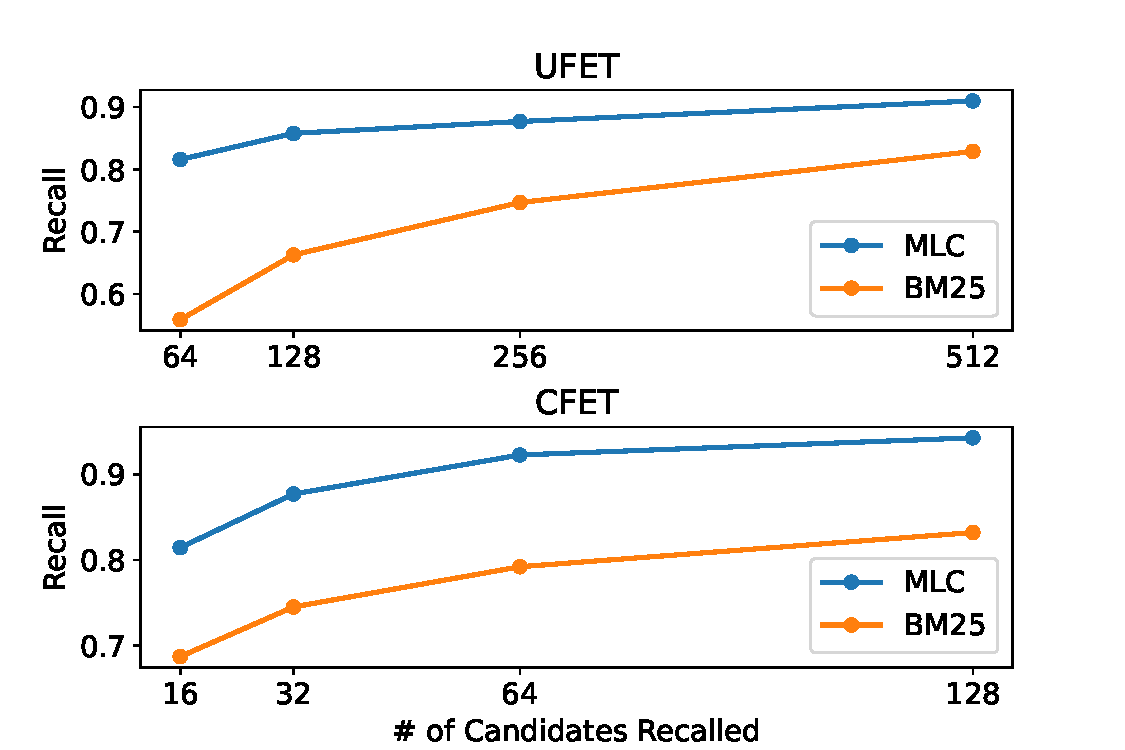
\includegraphics[width=\textwidth]{src/img/recall_compare_bm25.pdf}
         \label{fig:mb2}
     \end{subfigure}   
 \caption{Recall@$K$ of MLC and BM25.}
 \label{fig:recall}
\end{figure}

\subsection{Expand Stage}
\label{sec:expand}
In Table \ref{tab:expand}, we evaluate the F1 scores of all candidates expanded by exact match, and top-$10$ candidates expanded by the MLM using Bert-large. We also demonstrate the improvement of recall by using candidate expansion in Figure \ref{fig:expand_improvement}. On {\bf \textsc{UFET}} dataset, expanding around $32$ additional candidates based on $112$ MLC candidates results in $2\%$ higher recall compared to recalling all $128$ candidates by MLC. The recall of $128$ candidates after the expansion is comparable to the recall of $180$ candidates recalled from MLC. Similarly, expanding $10$ candidates is comparable to additionally recalling $80$ candidates using MLC.
In our experiments, we replace the last $48$ candidates recalled by MLC with the candidates recalled by MLM and Exact match for {\bf \textsc{UFET}} and $10$ for {\bf \textsc{CFET}}. We found the expand stage has a positive effect on the final performance of {\bf \textsc{\name}}s, and helps them reach SOTA performance (analyze in Sec. \ref{sec:analyze}).


\begin{table}[t]
\centering
\scalebox{0.75}{
\begin{tabular}{cccccc} 
\toprule
{\bf \textsc{Dataset}} & {\bf \textsc{Expand}} &   {\bf \textsc{P}}  & {\bf \textsc{R}}  &  {\bf \textsc{F1}} & \small{Avg \# Expanded}  \\ \midrule
\multirow{2}{*}{\bf \textsc{UFET}} & {\bf \textsc{Match}}      & 11.2   & 11.3     & 9.8    & 5.23     \\
      & {\bf \textsc{MLM}}  &  8.5     &   17.1   &  10.7  &    10    \\ \midrule
\multirow{2}{*}{\bf \textsc{CFET}} & {\bf \textsc{Match}}   &  11.4  &  14.5  & 11.2   & 4.57    \\
 & {\bf \textsc{MLM}}  & 21.3   &  19.5  & 17.7    & 10    \\ \midrule
\end{tabular}}
\caption{Evaluation of the recalled candidates.}
\label{tab:expand}
\end{table}
\begin{figure}[t]
     \centering
     \begin{subfigure}[h]{0.45\textwidth}
         \centering
         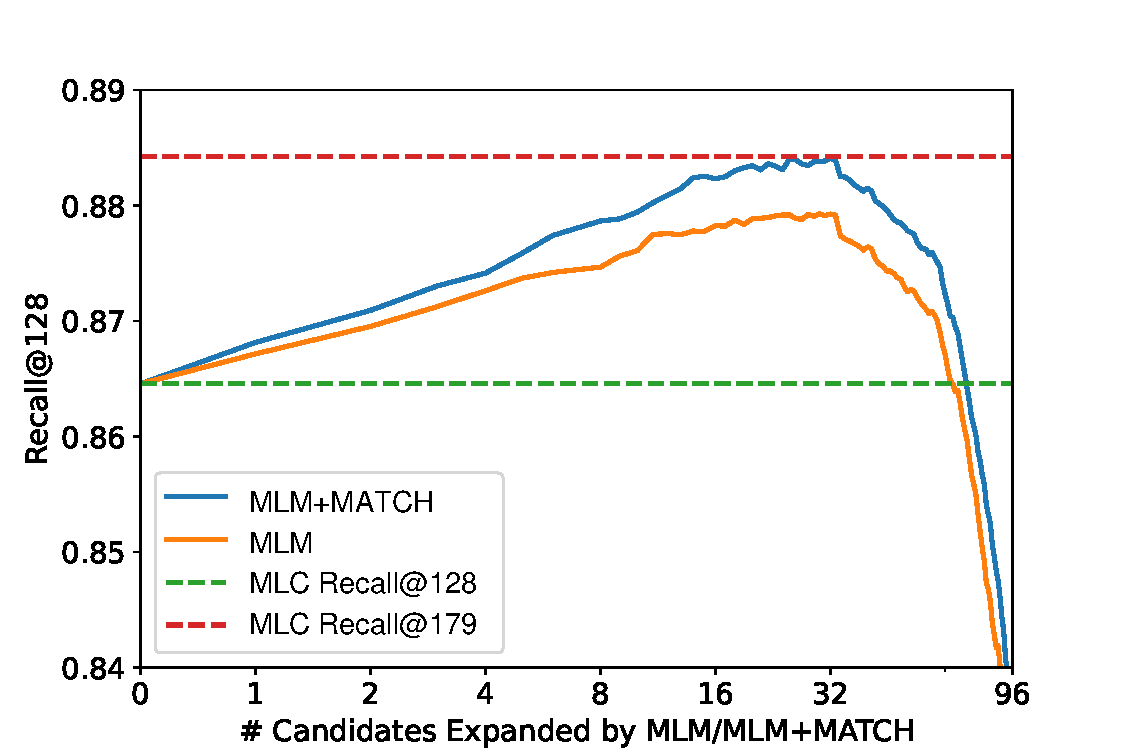
\includegraphics[width=\textwidth]{src/img/recall_ufet.pdf}
         \caption{Recall@$128$ on {\bf \textsc{UFET}} by including different number of expanded candidates. }
         \label{fig:c1}
     \end{subfigure}
     \vfill
     \begin{subfigure}[h]{0.45\textwidth}
         \centering
         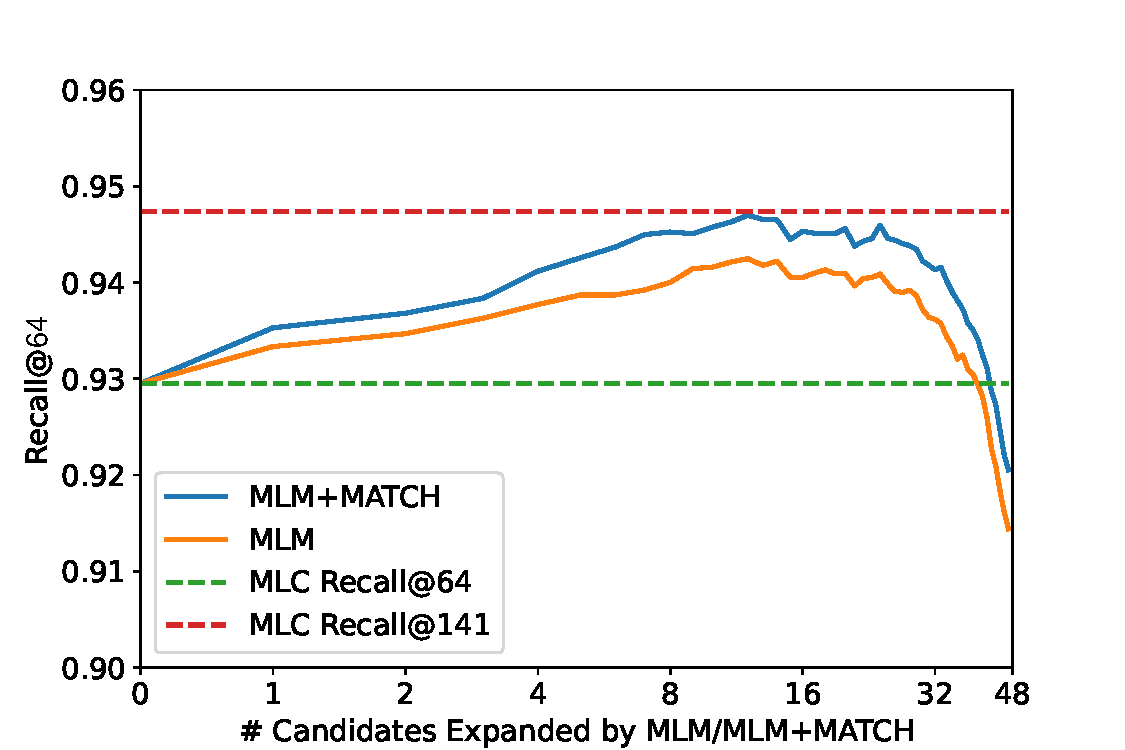
\includegraphics[width=\textwidth]{src/img/recall_cfet.pdf}
         \caption{Recall@$64$ on {\bf \textsc{CFET}} by including different number of expanded candidates.}
         \label{fig:c2}
     \end{subfigure}
\caption{Demonstration of the effect of expand stage. $x$-axis represents the number of candidates expanded by MLM/MLM+MATCH among these $128$ candidates. }
\label{fig:expand_improvement}
\end{figure}
\label{sec:exp_expand}
\subsection{Filter Stage and Final Results.}
\begin{table}[h!]
\centering
\scalebox{0.73}{
\renewcommand{\arraystretch}{1}
\begin{tabular}{cllll} \toprule
\multicolumn{2}{l}{\bf \textit{Base Models on UFET} }     & \bf \textsc{P}    & \bf \textsc{R}   & \bf \textsc{F1}  \\ \midrule
\multicolumn{5}{l}{\emph{MLC-like models}}        \\
\color{blue} \bf \texttt{B}& {\bf \textsc{Box4Types}}\cite{box4types}  & 52.8 & 38.8 & 44.8  \\
\color{blue}\bf \texttt{B}& {\bf \textsc{LDET}}$^\dagger$  \cite{onoe-durrett-2019-learning}          & 51.5 & 33.0 & 40.1 \\ 
\color{blue}\bf \texttt{B}& {\bf \textsc{MLMET}}$^\dagger$   {\cite{mlmet}}   & 53.6 & 45.3 & 49.1  \\
\color{blue}\bf \texttt{B}& {\bf \textsc{PL}}  \cite{ding2021prompt}   & 57.8 & 40.7 & 47.7 \\
\color{blue}\bf \texttt{B}& {\bf \textsc{DFET}}    \cite{dfet}      & 55.6 & 44.7 & 49.5 \\
\color{blue}\bf \texttt{B}& {\bf \textsc{MLC}} (reimplemented by us) & 46.5 & 34.9 & 39.9 \\ 
\color{red}\bf \texttt{R}& {\bf \textsc{MLC}} (reimplemented by us) & 42.2 & 44.9 & 43.5 \\ \hline 
\multicolumn{5}{l}{\emph{Seq2seq based models}}      \\
\color{blue}\bf \texttt{B} & {\bf \textsc{LRN} }  {\cite{liu-etal-2021-fine}}              & 54.5 & 38.9 & 45.4  \\\hline
\multicolumn{5}{l}{\emph{Filter models under our recall-expand-filter paradigm}}      \\
\color{blue}\bf \texttt{B} & {\bf \textsc{Vanilla CE}$_{128}$}   & 47.2 & 48.5 & 47.8 \\ 
\color{blue}\bf \texttt{B} & {\bf \textsc{\name-S$_{128}$}} (Ours)  & 53.2 & 48.3 & {\bf 50.6} \\ 
\color{blue}\bf \texttt{B} & {\bf \textsc{\name-S$_{128}$ w/o C2C}}   (Ours)   & 52.3 & 48.3 & 50.2 \\ 
\color{blue}\bf \texttt{B} & {\bf \textsc{\name-B$_{128}$}} (Ours)    & 49.9 & 50.0 & 49.9 \\ 
\color{blue}\bf \texttt{B} & {\bf \textsc{\name-B$_{128}$ w/o C2C}} (Ours)     & 49.9 & 48.2 & 49.0 \\ \hline
\color{red}\bf \texttt{R} & {\bf \textsc{Vanilla CE}$_{128}$}   & 49.6 & 49.0 & 49.3 \\ 
\color{red}\bf \texttt{R} & {\bf \textsc{\name-S$_{128}$}} (Ours)  & 53.3 & 47.3 & 50.1 \\ 
\color{red}\bf \texttt{R} & {\bf \textsc{\name-S$_{128}$ w/o C2C}}   (Ours)  & 53.2 & 46.6 & 49.7 \\ 
\color{red}\bf \texttt{R} & {\bf \textsc{\name-B$_{128}$}} (Ours)  & 52.5 & 47.9 & 50.1 \\ 
\color{red}\bf \texttt{R} & {\bf \textsc{\name-B$_{128}$ w/o C2C}} (Ours)     & 52.7 & 46.4 & 49.3 \\ \hline
\midrule
\multicolumn{2}{l}{\bf \textit{Large Models on UFET} }     & \bf \textsc{P}    & \bf \textsc{R}   & \bf \textsc{F1}  \\ \midrule
\multicolumn{5}{l}{\emph{MLC-like models}}        \\
\color{red}\bf \texttt{R} & {\bf \textsc{MLC}}  \cite{npcrf}               & 47.8 & 40.4 & 43.8  \\
\color{red}\bf \texttt{R} & {\bf \textsc{MLC-NPCRF}} \cite{npcrf}             & 48.7 & 45.5 & 47.0  \\
\color{red}\bf \texttt{R} & {\bf \textsc{MLC-GCN}} \cite{xiong-etal-2019-imposing}     & 51.2 & 41.0 & 45.5 \\
\color{blue}\bf \texttt{B} & {\bf \textsc{PL}}  \cite{ding2021prompt}       & 59.3 & 42.6 & 49.6  \\
\color{blue}\bf \texttt{B} & {\bf \textsc{PL-NPCRF}}  \cite{npcrf}  & 55.3 & 46.7 & {50.6}\\ \hline
\multicolumn{4}{l}{\emph{Cross-encoder based models and {\bf \textsc{\name}}s}}      \\
\color{red}\bf \texttt{R} & {\bf \textsc{LITE+L}}  \cite{lite}             & 48.7 & 45.8 & 47.2  \\
\color{teal}\bf \texttt{RM} & {\bf \textsc{LITE+NLI+L}} \cite{lite} & 52.4 & 48.9 & {50.6} \\ \hline
\multicolumn{4}{l}{\emph{Filter models under our recall-expand-filter paradigm}}   \\ 
\color{blue}\bf \texttt{B} & {\bf \textsc{Vanilla CE$_{128}$}}   & 50.3 & 49.6 & 49.9 \\ 
\color{blue}\bf \texttt{B} & {\bf \textsc{\name-S$_{128}$}}  (Ours)   & 52.5 & 49.1 & 50.8 \\ 
\color{blue}\bf \texttt{B} & {\bf \textsc{\name-S$_{128}$ w/o C2C}}   (Ours)   & 54.1 & 47.1 & 50.4 \\ 
\color{blue}\bf \texttt{B} & {\bf \textsc{\name-B$_{128}$}} (Ours)    & 54.0 & 48.6 & 51.2 \\ 
\color{blue}\bf \texttt{B} & {\bf \textsc{\name-B$_{128}$ w/o C2C}} (Ours)     & 52.8 & 48.3 & 50.4 \\ \hline
\color{red}\bf \texttt{R} & {\bf \textsc{Vanilla CE$_{128}$}}   & 54.5 & 49.3 & 51.8 \\ 
\color{red}\bf \texttt{R} & {\bf \textsc{\name-S$_{128}$}}  (Ours)   & 50.8 & 49.8  &  50.3 \\ 
\color{red}\bf \texttt{R} & {\bf \textsc{\name-S$_{128}$ w/o C2C}}   (Ours)   & 51.5 & 48.8 & 50.1 \\ 
\color{red}\bf \texttt{R} & {\bf \textsc{\name-B$_{128}$}} (Ours)    & 51.9 & 50.8 & 51.4 \\ 
\color{red}\bf \texttt{R} & {\bf \textsc{\name-B$_{128}$ w/o C2C}} (Ours)     & 51.6 & 51.6 & 51.6 \\ \hline
\color{teal}\bf \texttt{RM} & {\bf \textsc{\name-B$_{128}$ w/o C2C}} (Ours) & 56.3 & 48.5 & {\bf 52.1} \\ \hline
\midrule
\end{tabular}}
\caption{Macro-averaged UFET result. {\bf \textsc{LITE+L}} is LITE without NLI pretraining, {\bf \textsc{LITE+L+NLI}} is the full LITE model. Methods marked by $\dagger$ utilize either distantly supervised or augmented data for training. {\bf \textsc{\name-S$_{128}$}} denotes we use $128$ candidates recalled and expanded from the first two stages.}
\label{tab:ufet}
\end{table}
\begin{table}[t]
\centering
\scalebox{0.75}{
\renewcommand{\arraystretch}{1}
\begin{tabular}{cllll} \toprule
\multicolumn{2}{l}{\bf \textit{Models on CFET} }     & \bf \textsc{P}    & \bf \textsc{R}   & \bf \textsc{F1}  \\ \midrule
\multicolumn{5}{l}{\emph{MLC-like models}}        \\
\color{purple}\bf \texttt{N}& {\bf \textsc{MLC}} & 55.8 & 58.6 & 57.1 \\  
\color{purple}\bf \texttt{N}& {\bf \textsc{MLC-NPCRF}} \cite{npcrf}     & 57.0 & 60.5 & 58.7 \\ 
\color{purple}\bf \texttt{N}& {\bf \textsc{MLC-GCN}} \cite{xiong-etal-2019-imposing}   & 51.6 & 63.2 & 56.8 \\ 
\color{brown}\bf \texttt{C}& {\bf \textsc{MLC}} & 54.0 & 59.5 & 56.6 \\  
\color{brown}\bf \texttt{C}& {\bf \textsc{MLC-NPCRF}} \cite{npcrf}   & 54.0 & 61.6 & 57.3 \\  
\color{brown}\bf \texttt{C}& {\bf \textsc{MLC-GCN}} \cite{xiong-etal-2019-imposing} & 56.4 & 58.6 & 57.5 \\ \midrule 
\multicolumn{5}{l}{\emph{Filter models under our recall-expand-filter paradigm}}      \\
\color{purple}\bf \texttt{N} & {\bf \textsc{Vanilla CE}}   & 57.6 & 64.3 & 60.7 \\ 
\color{brown}\bf \texttt{C} & {\bf \textsc{Vanilla CE}}   & 54.0 & 63.3 & 58.3 \\  \hline
\color{purple}\bf \texttt{N} & {\bf \textsc{\name-S$_{64}$}} (Ours)  & 58.4 & 62.1 & 60.2 \\ 
\color{purple}\bf \texttt{N} & {\bf \textsc{\name-S$_{64}$ w/o C2C}}   (Ours)   & 59.1 & 61.5 & 60.3 \\ 
\color{purple}\bf \texttt{N} & {\bf \textsc{\name-B$_{64}$}} (Ours)    & 56.7 & 66.1 & 61.1 \\ 
\color{purple}\bf \texttt{N} & {\bf \textsc{\name-B$_{64}$ w/o C2C}} (Ours)     & 58.8 & 64.1 & 61.4 \\ \hline
\color{brown}\bf \texttt{C} & {\bf \textsc{\name-S$_{64}$}} (Ours)  & 55.5 & 62.6 & 58.8 \\ 
\color{brown}\bf \texttt{C} & {\bf \textsc{\name-S$_{64}$ w/o C2C}}   (Ours)   & 54.0 & 63.4 & 58.3 \\ 
\color{brown}\bf \texttt{C} & {\bf \textsc{\name-B$_{64}$}} (Ours)    & 55.0 & 63.5 & 59.0 \\ 
\color{brown}\bf \texttt{C} & {\bf \textsc{\name-B$_{64}$ w/o C2C}} (Ours)     & 57.3 & 61.3 & 59.3 \\ \hline
\midrule
\end{tabular}}
\caption{Macro-averaged CFET result.}
\label{tab:cfet}
\end{table}

In this section, we report the performance of {\bf \textsc{MCCE}} variants as the filter models and compare them with various strong baselines that we will introduce later. We also compare the inference speed of different models in this section. For filter models, we treat the number of candidates $K$ recalled and expanded by the first two stages as hyper-parameters, and tune it on the development set. We found the choice of PLM backbones has a non-negligible effect on the performance, and the PLM backbone of previous methods varies. Therefore for fairer comparisons to baselines, we conduct experiments of {\bf \textsc{\name}} using different backbone PLMs for our {\bf \textsc{\name}} models and report the results. For all {\bf \textsc{\name}} models, we use AdamW optimizer with a learning rate tuned between $5\times 10^{-6}$ and $2\times 10^{-5}$. The batch size we use is $4$ and we train the models for at most $50$ epochs with early stopping. {\bf \textsc{UFET}} also provides a large dataset obtained from distant supervision such as entity linking, we do not use it and only train and evaluate our models on human-labeled data.
\paragraph{Baselines}
The {\bf \textsc{MLC}} model we used for the recall stage and the cross-encoder ({\bf \textsc{CE}}) we introduced in Sec. \ref{sec:vanilla_ce} are natural baselines. We also compare our methods with recent PLM-based methods. {\bf \textsc{LDET} }\cite{onoe-durrett-2019-learning} is an MLC with Bert-base-uncased and ELMo \cite{elmo} trained on 727k examples automatically denoised from the distantly labeled UFET. {\bf \textsc{GCN} }\cite{xiong-etal-2019-imposing} uses GCN to model type correlations and obtain type embeddings. Types are scored by dot-product of mention and type embeddings. The original paper uses BiLSTM as the mention encoder and we use the results re-implemented by \citet{npcrf} using RoBERTa-large. {\bf \textsc{Box4Type} }\cite{box4types} uses Bert-large as the backbone and uses box embedding to encode mentions and types for training and inference. {\bf \textsc{LRN} }\cite{liu-etal-2021-fine} use Bert-base as the encoder and an LSTM decoder to generate types in a seq2seq manner. {\bf \textsc{MLMET} }\cite{mlmet} is a {\bf \textsc{MLC}} with Bert-base, but first pretrained by the distantly-labeled data augmented by masked word prediction, then finetuned and self-trained on the 2k human-annotated data. {\bf \textsc{PL}} \cite{ding2021prompt} uses prompt learning for entity typing. {\bf \textsc{DFET} }\cite{dfet} uses {\bf \textsc{PL}} as backbone and is a multi-round automatic denoising method for 2k labeled data. {\bf \textsc{LITE} }\cite{lite} is the previous SOTA system that formulates entity typing as textual inference. {\bf \textsc{LITE}} uses RoBERTa-large-MNLI as the backbone, and is a cross-encoder (introduced in Sec. \ref{sec:vanilla_ce}) with designed templates and a hierarchical loss. \citet{npcrf} proposes {\bf \textsc{NPCRF}} to enhance backbones such as {\bf \textsc{PL}} and {\bf \textsc{MLC}} by modeling type correlations, and reach performance comparable to {\bf \textsc{LITE}}.

\paragraph{Naming Conventions}
Let {\bf \textsc{\name-S}} be the {\bf \textsc{\name}} model that treats candidates as sub-tokens, and {\bf \textsc{\name-B}} be the model representing candidates as fixed-size blocks. The {\bf \textsc{\name}} model without {\bf \textsc{C2C}} attention (mentioned in Sec. \ref{sec:attn}) is denoted as {\bf \textsc{\name-B} w/o C2C}. For PLM backbones used in {\bf \textsc{UFET}}, we use {\color{blue} \bf \texttt{B}}, {\color{red} \bf \texttt{R}}, {\color{teal} \bf \texttt{RM}} to denote BERT-base-cased \cite{bert}, RoBERTa \cite{liu2019roberta}, and RoBERTa-MNLI \cite{liu2019roberta} respectively. For {\bf \textsc{CFET}}, we adopt two widely-used Chinese PLM, BERT-base-Chinese and NeZha-base-Chinese, and denote them as {\color{brown} \bf \texttt{C}} and {\color{purple} \bf \texttt{N}} respectively. 

\paragraph{UFET Results} We show the results of {\bf \textsc{UFET}} dataset in Table \ref{tab:ufet}. The results show that: (1) The recall-expand-filter paradigm is effective. Filter models outperform all baselines without the paradigm by a large margin. The vanilla CE under our paradigm reaches $51.8$ F1 compared to more complexed CE {\bf \textsc{LITE}} with $50.6$ F1 (2) {\bf \textsc{\name}} models reach SOTA performances. {\bf \textsc{\name-S$_{128}$}} with BERT-base performs best and reaches {\bf 50.6} F1 score, which is comparable to previous SOTA performance of large models such as {\bf \textsc{LITE+NLI+L}} and {\bf \textsc{PL+NPCRF}}. Among large models, {\bf \textsc{\name-B$_{128}$ w/o C2C}} also reaches SOTA performance with {\bf 52.1} F1 score. (3) {\bf \textsc{C2C}} attention is not necessary on large models, but is useful in base models. (4) Large models can utilize type semantics better. We found {\bf \textsc{\name-B}} outperforms {\bf \textsc{\name-S}} on large models, but underperforms {\bf \textsc{\name-S}} on base models. (5) Backbone PLM matters. We found the performance of {\bf \textsc{Vannila CE}} under our paradigm is largely affected by the PLM it used. It reaches $47.8$ F1 with BERT-base and $51.8$ F1 with RoBERTa-large. For {\bf \textsc{\name}} models, we found {\bf \textsc{\name}} performs better than {\bf \textsc{\name-B}} with BERT, and worse than {\bf \textsc{\name-B}} with RoBERTa. 

\begin{table*}[t]
\centering
\scalebox{0.9}{
\begin{tabular}{lllcc} \toprule
\bf \textsc{Model}  & \bf \textsc{\# FP} & \bf \textsc{Attn} & \bf \textsc{sents/sec} & \bf \textsc{F1} \\ \midrule
{\bf \textsc{MLC}} & \small{$1$}  & \small{$L_S^2D$} & 58.8 & 43.8\\
{\bf \textsc{LITE+NLI+L (CE)}}  & \small{$N$}  & \small{$L_S^2D$} & 0.02 & 50.6\\ \midrule \hline
\multicolumn{5}{l}{\emph{filter stage inference speed.}}  \\
{\bf \textsc{Vanilla CE$_{128}$}}  & \small{$128$}  & \small{$L_S^2D$} & 1.64 & 51.8 \\ 
{\bf \textsc{\name-S$_{128}$}}  & \small{$1$}  & \small{$(L_S+128)^2D$} & 60.8 & 50.1 \\ 
{\bf \textsc{\name-B$_{128}$}}  & \small{$1$}  & \small{$(L_S+128B)^2D$} & 22.3 & 51.4\\ 
{\bf \textsc{\name-B$_{128}$ w/o C2C}}  & \small{$1$}  & \small{$(L_S^2+256L_S B + 128 B^2)D$} & 25.2 & {\bf 52.1}\\ \bottomrule
\end{tabular}}
\caption{Inference speed comparison of models. {\bf \textsc{\# FP}} means the number of PLM forward passes required by a single inference. {\bf \textsc{ATTN}} column lists the theoretical attention complexity.  We also report the practical inference speed {\bf \textsc{sents/sec}} and the {\bf \textsc{F1}} scores on {\bf \textsc{UFET}} with RoBERTa-large architecture.}
\label{tab:speed}
\end{table*}

\begin{table}[t]
\centering
\scalebox{0.85}{
\renewcommand{\arraystretch}{1}
\begin{tabular}{cllll} \toprule
\multicolumn{2}{l}{\bf \textit{Models} }     & \bf \textsc{P}    & \bf \textsc{R}   & \bf \textsc{F1}  \\ \midrule
\multicolumn{5}{l}{\emph{coarse (9 types) Open Entity}}        \\ \hline
\color{red}\bf \texttt{R} & {\bf \textsc{MLC}}   & 76.8 & 78.5 & 77.6 \\ 
\color{red}\bf \texttt{R} & {\bf \textsc{Vanilla CE$_{9}$}}   & 82.3 & 81.0 & 81.6 \\ 
\color{red}\bf \texttt{R} & {\bf \textsc{\name-S$_{9}$}}   & 77.0 & 87.7 & 82.0 \\ 
\color{red}\bf \texttt{R} & {\bf \textsc{\name-B$_{9}$ w/o C2C}}   & 77.2 & 85.4 & 81.1 \\ \hline
\multicolumn{5}{l}{\emph{fine (130 types)}}        \\ \hline
\color{red}\bf \texttt{R} & {\bf \textsc{MLC}}   & 70.4 & 63.7 & 66.9  \\ 
\color{red}\bf \texttt{R} & {\bf \textsc{Vanilla CE}$_{130}$}   & 67.9 & 66.4 & 67.1 \\ 
\color{red}\bf \texttt{R} & {\bf \textsc{\name-S$_{130}$}}   & 65.8 & 71.8 & 68.7 \\ 
\color{red}\bf \texttt{R} & {\bf \textsc{\name-B$_{130}$ w/o C2C}}   & 64.1 & 70.5 & 67.1 \\ \hline
\midrule
\end{tabular}}
\caption{Micro-averaged results on UFET fine and coarse.}
\label{tab:ufet-coarse-fine}
\end{table}

\paragraph{CFET Results} We conduct experiments on {\bf \textsc{CFET}} and compare {\bf \textsc{\name}} models with several strong baselines:  {\bf \textsc{NPCRF}} and {\bf \textsc{GCN}} with MLC-like architecture, and {\bf \textsc{Vanilla CE}} under out paradigm which is proved to be better than {\bf \textsc{LITE}} on {\bf \textsc{UFET}}. The results are shown in Table \ref{tab:cfet}. Similar to results in {\bf \textsc{UFET}}, filter models under our paradigm significantly outperform MLC-like baselines, $+2.0$ F1 for Nezha-base and $+1.8$ F1 for BERT-base-Chinese. In {\bf \textsc{CFET}}, {\bf \textsc{\name}-B} is significantly better than {\bf \textsc{\name}-S}, on both Nezha-base and BERT-base-Chinese, indicating the importance of type semantics in Chinese language. We also find that {\bf \textsc{\name} w/o C2C} is generally better than  {\bf \textsc{\name} w/ C2C}, it is possibly because the C2C attention distracts the candidates from attending to mention and contexts.
\paragraph{Speed Comparison} Table \ref{tab:speed} shows the theoretical inference complexity (number of PLM forward passes, and attention complexity), and practical inference speed (number of sentences inferred per second) of different models. We conduct the speed test using NVIDIA TITAN RTX for all models, and the inference batch size is 4.
At the filter stage, the inference speed of {\bf \textsc{\name-S}} is on par with {\bf \textsc{MLC}} (even slightly faster because we don't need to score all types), and is about 40 times faster than {\bf \textsc{Vannila CE}} and thousands of times faster than {\bf \textsc{LITE}}. {\bf \textsc{\name-B w/o C2C}} is not significantly faster than {\bf \textsc{\name-B}} as expected. It's possibly because the computation related to the block attention is not fully optimized by existing deep learning frameworks. The speed advantage of {\bf \textsc{\name-B w/o C2C}} over {\bf \textsc{\name-B}} will be greater with more candidates.


\subsection{Fine-grained and Coarse-grained Entity Typing}
We also conduct experiments on Fine-grained (130-class) and Coarse-grained (9-class, also known as ``Open Entity'') entity typing, and the results are shown in Table \ref{tab:ufet-coarse-fine}. As the type candidate set is much smaller in these settings, we skip the recall and expand stages and directly run the filter models and compare them to baselines. Results show that both {\bf \textsc{\name}-S} and {\bf \textsc{\name}-B} are still better than {\bf \textsc{MLC}} and {\bf \textsc{Vanilla CE}}, and {\bf \textsc{\name}-S} is better than {\bf \textsc{\name}-B} on coarser-grained cases possibly because the coarser-grained types are simpler in surface-forms and {\bf \textsc{\name}-S} will not lose many type semantics.






\section{Discussion and Future Works}
In addition to the general adversarial evaluation framework \advcodec, this paper also aims to explore several scientific questions: 1)  Since \advcodec allows the flexibility of manipulating at different levels of a tree hierarchy, which level is more attack effective and which one preserves better grammatical correctness? 2) Is it possible to achieve the targeted attack for general NLP tasks such as sentiment classification and QA, given the limited degree of freedom for manipulation? 3) Is it possible to perform a blackbox attack for many  NLP tasks? 4) Is BERT robust in practice? 
5) Do these adversarial examples affect human reader performances? 
%\boxin{I think the above question is readers caring more. 5) Are human readers more sensitive to an appended adversarial sentence or scatter of added words?

% To address the above questions, we generate adversarial text against different models of sentiment classification and QA in each encoding scenario. Compared with the state-of-the-art adversarial text generation methods, our approach achieves significantly higher untargeted and \emph{targeted} attack success rate. In addition, we perform both whitebox and transferability-based blackbox settings to evaluate the model vulnerabilities. 
% Within each attack setting, we quantitatively evaluate the attack effectiveness of different attack strategies, including appending an additional adversarial sentence and adding scatter of adversarial words to a paragraph.
% To provide thorough adversarial text quality assessment, we also perform 7 groups of human studies to evaluate the quality of the generated adversarial text. % Compared with the baselines methods, and whether a human can still get the ground truth answers for these tasks based on adversarial text.

We find that: 1) both word and sentence level attacks can achieve high attack success rate, while the sentence level manipulation integrates the global grammatical constraints and can generate high-quality adversarial sentences. 2) various targeted attacks on general NLP tasks are possible (\textit{e.g.}, when attacking QA, we can ensure  the target to be a specific answer or a specific location within a sentence); 3) the transferability based blackbox attacks are successful in NLP tasks. 
% Transferring adversarial text from stronger models (in terms of performances) to weaker ones is more successful; 
4)  Although BERT has achieved state-of-the-art performances, we observe the performance drops are also more substantial than other models when confronted with adversarial examples, which indicates BERT is not robust enough under the adversarial settings.
%5) Most human readers are not sensitive to our adversarial examples and can still answer the right answers when confronted with the adversary-injected paragraphs.

Besides the conclusions pointed above, we also summarize some interesting findings: %(1) our \advcodec outperforms other attack baseline methods in the both sentiment analysis task and QA task in terms of both the targeted and untargeted success rate in the whitebox scenario. 
(1) While \advcodecword achieves the best attack success rate among multiple tasks, we observe a trade-off between the freedom of manipulation and the attack capability. For instance, \advcodecsent has dependency tree constraints and becomes more natural for human readers than but less effective to attack models than \advcodecword. Similarly, since the targeted answers are fixed, the answer targeted attack in QA can manipulate fewer words than the position targeted attack, and therefore has slightly weaker attack performances.
% (2) Scatter attack is as effective as concat attack in sentiment classification task but less successful in QA, because QA systems make decisions highly based on the contextual correlation between the question and the paragraph, which makes it difficult to set an arbitrary token as our targeted answer.
(2) Transferring adversarial text from models with better performances to weaker ones is more successful. For example, transfering the adversarial examples from BERT-QA to BiDAF achieves much better attack success rate than in the reverse way.
(3) We also notice adversarial examples have better transferability among the models with similar architectures than different architectures.
(4) BERT models give higher attention scores to the both ends of the paragraphs and tend to overlook the content in the middle, as shown in \S \ref{sec:ablation} ablation study that adding adversarial sentences in the middle of the paragraph is less effective than in the front or the end.

To defend against these adversaries, here we discuss about the following possible methods and will in depth explore them in our future works: 
(1) \textbf{Adversarial Training} is a practical methods to defend against adversarial examples. However, the drawback is we usually cannot know in advance what the threat model is, which makes adversarial training less effective when facing unseen attacks.
(2) \textbf{Interval Bound Propagation} (IBP) \citep{Dvijotham2018TrainingVL} is proposed as a new technique to theoretically consider the worst-case perturbation. Recent works \citep{Jia2019CertifiedRT,Huang2019AchievingVR} have applied IBP in the NLP domain to certify the robustness of models. (3) \textbf{Language models} including GPT2 \citep{Radford2019LanguageMA} may also function as an anomaly detector to probe the inconsistent and unnatural adversarial sentences.

%Besides the conclusions pointed out in the \S \ref{sec:intro}, we also summarize some interesting findings: %(1) our \advcodec outperforms other attack baseline methods in the both sentiment analysis task and QA task in terms of both the targeted and untargeted success rate in the whitebox scenario. 
%(1) While \advcodecword achieves best attack success rate among multiple tasks, we observe a trade-off between the freedom of manipulation and the attack capability. For instance, \advcodecsent has dependency tree constraints and becomes more natural for human readers than but less effective to attack models than \advcodecword. Similarly, the answer targeted attack in QA has fewer words to manipulate and change than the position targeted attack, and therefore has slightly weaker attack performances.
%(2) Scatter attack is as effective as concat attack in sentiment classification task but less successful in QA, because QA systems make decisions highly based on the contextual correlation between the question and the paragraph, which makes it difficult to set an arbitrary token as our targeted answer.
% (3) Transferring adversarial text from models with better performances to weaker ones is more successful. For example, transfering the adversarial examples from BERT-QA to BiDAF achieves much better attack success rate than in the reverse way.
% (4) We also notice adversarial examples have better transferability among the models with similar architectures than different architectures.
% (5) BERT models give higher attention scores to the both ends of the paragraphs and tend to overlook the content in the middle, as shown in \S \ref{sec:ablation} ablation study that adding adversarial sentences in the middle of the paragraph is less effective than in the front or the end.

% To defend against these adversaries, here we discuss about the following possible methods and will in depth explore them in our future works: 
% (1) \textbf{Adversarial Training} is a practical methods to defend against adversarial examples. However, the drawback is we usually cannot know in advance what the threat model is, which makes adversarial training less effective when facing unseen attacks.
% (2) \textbf{Interval Bound Propagation} (IBP) \citep{Dvijotham2018TrainingVL} is proposed as a new technique to theoretically consider the worst-case perturbation. Recent works \citep{Jia2019CertifiedRT,Huang2019AchievingVR} have applied IBP in the NLP domain to certify the robustness of models. (3) \textbf{Language models} including GPT2 \citep{Radford2019LanguageMA} may also function as an anomaly detector to probe the inconsistent and unnatural adversarial sentences.

%(2) We can clearly observe a tradeoff between the degree of freedom for manipulation and attack success rate. For example, we observe a small drop in the attack success rate for answer targeted attack compared to position targeted attack, due to the fact that we put more constraints to ensure pre-specified answer targets unchanged in the optimization process. Similarly, the dependency tree constraints turn out to be more strong and harsh constraints on the adversarial sentences, thus achieving higher language quality at the cost of  attack success rate. 
%(2)
%(3) \boxin{How to say because our transfer based blackattack does not beat AddSent because it is input-agnoistic.? while ours are more model-specific?}  (4) BERT based sentiment classifier is more vulnerable than standard sentiment classifier, while BERT based QA model is more robust and harder to attack than the widely-used QA model.
% \vspace{-2mm}
\section{Conclusions}
In summary, we propose a general targeted attack framework for adversarial text generation. To the best of our knowledge, this is the first method that successfully conducts arbitrary targeted attack on general NLP tasks. %In addition to the core methodological contribution, this paper also conducts extensive data experiments and human evaluation to obtain and confirm answers to several important scientific questions in NLP. 
Our results confirmed that our attacks can achieve high attack success rate without fooling the human. 
% We also find that compared to the more traditional machine learning methods,  BERT based sentiment classification and QA models are more vulnerable. 
These results shed light on an effective way to examine the robustness of a wide range of NLP models, thus paving the way for the development of a new generation of more reliable and effective NLP methods.
\section*{Acknowledgement}
This work is partially supported by NSF grant No.1910100, Amazon research award, DARPA No. HR00111990074. We thank the anonymous reviewers for their insightful comments.

\bibliographystyle{acl_natbib}
\bibliography{t3}
% \appendix
\section{Dynamic Smagorinsky Model}
\label{app:dynsmago}

Germano et al. proposed in \cite{germano1991dynamic} an improvement to the standard Smagorinsky model by setting the Smagorinsky constant $C_s$ not to a fixed value set a priori, but rather to adapt it dynamically in space and time dependent on the current state of the flow.
This dynamic procedure is based on applying a test filter $\widehat{(\cdot)}$ to the solution.
The LES solution can then be used to compute the resolved stress tensor
\begin{equation}
  L_{ij} = \widehat{\widetilde{u}_i \widetilde{u}_j} - \widehat{\widetilde{u}}_i \widehat{\widetilde{u}}_j,
\end{equation}
which entails the subgrid stresses induced by the test filter.
Germano's identity finds a correlation between those resolved subgrid stresses and the unknown subgrid stress induced by the LES filter.
Lilly \cite{lilly1992proposed} proposed a least-squares approach to compute $C_s^2$ such that Germano's identity is optimally obeyed, which gives
\begin{equation}
  C_s^2 = \frac{\langle L_{ij}M_{ij}\rangle_{avg}}{\langle M_{ij}M_{ij} \rangle_{avg}}.
  \label{eq:dynsmago_ls}
\end{equation}
Here, $\langle\cdot\rangle_{avg}$ denotes some averaging operation to avoid extremely large coefficients and thus to stabilize the model.
The tensor $M_{ij}$ is shorthand for the expression
\begin{equation}
  M_{ij} = 2 \Delta^2 \widehat{\sqrt{2\tilde{S}_{kl}\tilde{S}_{kl}}\,\tilde{S}_{ij}}  - 2 \widehat{\Delta}^2 \sqrt{2\widehat{\tilde{S}}_{kl}\widehat{\tilde{S}}_{kl}}\, \widehat{\tilde{S}}_{ij},
\end{equation}
with $\widehat{\Delta}$ as the filter width of the test filter and with the rate-of-strain tensor on the test filter level $\widehat{\tilde{S}}$ computed analogously to \eqref{eq:smago} based on the test-filtered velocity field $\widehat{\tilde{u_i}}$.

In the DG context, the dynamic procedure is applied in an elementwise fashion.
As test filter $\widehat{(\cdot)}$ with filter width $\widehat{\Delta}$, we apply a modal cut-off filter to the solution polynomial with a degree of $N_{test}=2$ and $N_{test}=3$ for the cases employing a polynomial degree of $N=5$ and $N=7$, respectively.
Moreover, the averaging operator $\langle\cdot\rangle_{avg}$ for the numerator and denominator in \eqref{eq:dynsmago_ls} is chosen as an average in each element yielding a single coefficient $C_s^2$ for each element.
The resulting eddy-viscosity is then clipped to the range $\mu_t \in [-100\mu,1000\mu]$ with respect to the physical viscosity, since the unclipped model produced from time to time a few huge values for $C_s^2$, which deteriorated the solution quite drastically.
The clipping range itself seemed to have only very limited influence on the model's behavior in our tests and provided very similar results for a wide range of different clipping intervals.

\end{document}
